\input{../preamble}
\input{../usercommands}

\begin{document}
\vspace*{2cm}

{\centerline{\bf\huge AST2000 Lecture Notes}}

\vspace*{1cm}

\newcommand{\PartName}{2C}
\newcommand{\refproblem}[1]{\PartName.\ref{#1}}


{\centerline{\bf\LARGE Part \PartName}}\vspace*{0.25cm}
{\centerline{\bf\LARGE General Relativity:  Basic principles}}

\vspace*{1cm}

{\centerline{\underline{\LARGE Questions to ponder before the lecture}}}

\vspace*{1cm}

{\large
\begin{enumerate}
\item What is a black hole? (how would you define it?)
\item If you, situated in a safe place far away from the black hole, see somebody falling into a black hole, what will you see?
\item If you instead are situated close to the black hole, will things look different?
\item In General Relativity the idea of a force of gravity is replaced by the curvature of spacetime. Based on what you learned in the lectures on special relativity, can you imagine what curved spacetime might mean?
\item A free-float frame in General Relativity is defined as a place where an object which is left with no velocity will continue with zero velocity. We know that this will happen in an intertial frame which is not affected by external forces. But can you imagine a situation where this is also the case in an accelerated frame?
\end{enumerate}

\begin{Figure}%[htb]
\centering
%\begin{center}
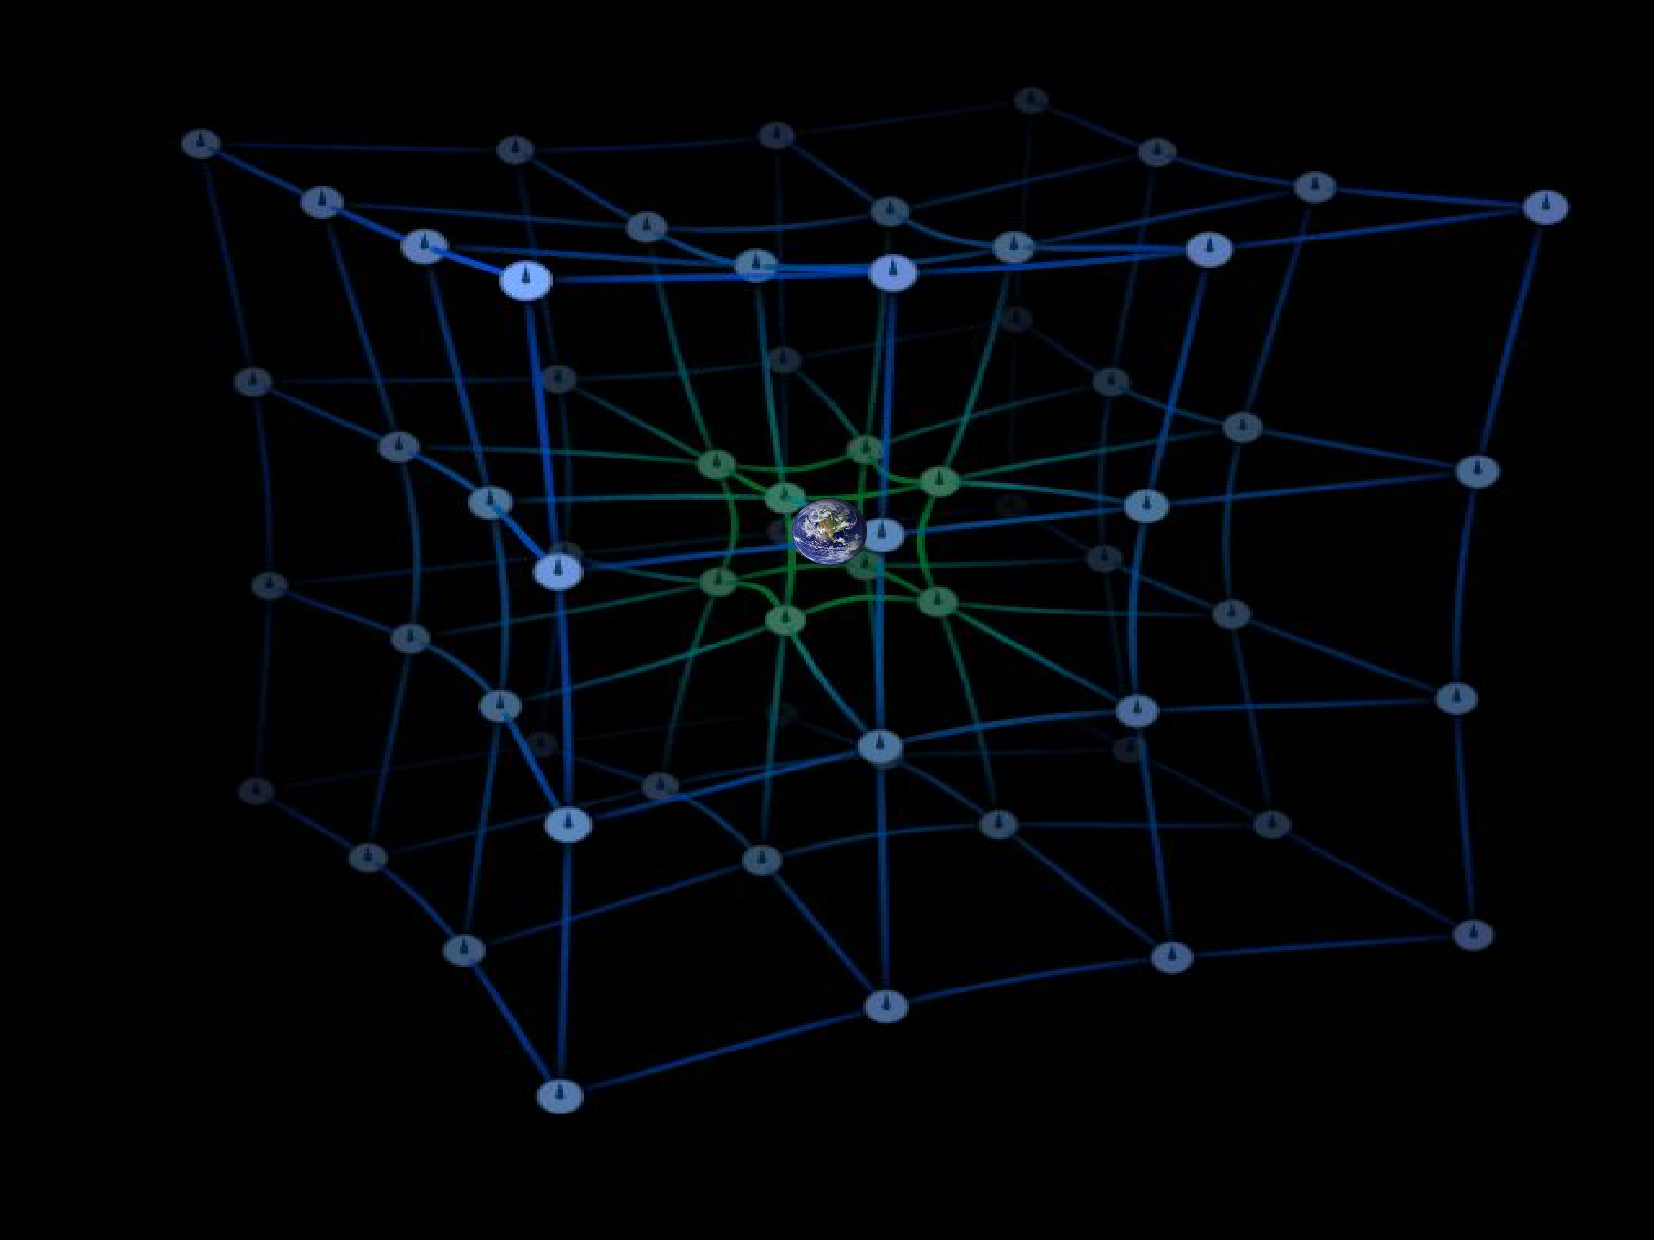
\includegraphics[width=0.72\textwidth]{spacetimebending.pdf}
%\end{center}
\end{Figure}
%Image: https://www.reddit.com/r/gifs/comments/4eaw4h/general_relativity_conceptual_illustration_of/ (modified)


\clearpage
\vspace*{2cm}

{\centerline{\bf\huge AST2000 Lecture Notes}}

\vspace*{1cm}

{\centerline{\bf\LARGE Part \PartName}}\vspace*{0.25cm}
{\centerline{\bf\LARGE General Relativity:  Basic principles}}

\vspace*{1cm}

\begin{multicols}{2}

\section{\ss geometry}
\label{sect:geometry}

The general theory of relativity may be summarized in one equation, the Einstein equation
\[
G_{\mu\nu}=8\pi T_{\mu\nu},
\]
where $G_{\mu\nu}$ is the Einstein tensor and $T_{\mu\nu}$ is the stress-energy tensor (A tensor is a matrix with particular properties in the same way as a 4-vector is a vector with specific properties). This equation is not a part of this course as tensor mathematics and linear algebra, not required for taking this course, are needed to understand it. I present it here anyway as it illustrates the basic principle of general relativity: The stress-energy tensor on the right hand side contains the energy content of spacetime, the Einstein tensor on the left hand side specifies the geometry of spacetime. Thus, general relativity says that the energy content in spacetime specifies its geometry. 

What do we mean by geometry of spacetime? We have already seen two examples of such geometries, Euclidean geometry and Lorentz geometry. We have also seen that the geometry is specified by the spacetime interval (also called {\it line element}) $\Delta s$ which tells us how distances are measured. Thus, by inserting the energy content as a function of spacetime coordinates on the right side, the left side gives us an expression for $\Delta s$, i.e.\ how to measure distances in spacetime in the presence of mass/energy. Thus, in the presence of a mass, for instance like the Earth, the geometry of spacetime is no longer Lorentz geometry and the laws of special relativity are no longer valid. This should be obvious: Special relativity tells us that a particle should follow a straight line in spacetime, i.e.\ a path with constant velocity. This is clearly not the case on Earth, objects do not keep a constant velocity, they accelerate with the gravitational acceleration. 

You might object here: Special relativity says that a particle continues with constant velocity if it is not influenced by external forces, but here the force of gravity is at play. The answer to this objection is given by a very important concept of general relativity: \emph{gravity is not a force}. What we experience as 'the force of gravity' is simply a result of the spacetime geometry in the vicinity of masses. The principle of maximal aging (go back and repeat it now!) tells us that a particle which is not influenced by external forces follows the longest path in spacetime, i.e.\ the path which gives the largest possible proper time. An object falls to the ground because the geometry of spacetime around a large mass like Earth is such, that when the object follows the path with the longest possible path length $\Delta s$, it falls to the ground. It does not continue in a straight line with constant velocity as it would in a spacetime with Lorentz geometry.


Few years after Einstein published the general theory of relativity, Karl \ss found a general solution to the Einstein equation for the geometry around an isolated spherically symmetric body. This is one of the very few analytic solutions to the Einstein equation that exists. Thus, the \ss solution is valid around a lonely star, planet or a black hole. The spacetime geometry resulting from this solution is called \ss geometry and is described by the line element:
\begin{formbox}
\textbf{The \ss line element}
\begin{equation}
\label{eq:ss}
\Delta s^2=\sst\Delta t^2-\frac{\Delta r^2}{\sst}-r^2\Delta\phi^2.
\end{equation}
\end{formbox}


\begin{figure*}
\fcolorbox{black}{yellow}{\parbox{\dimexpr \linewidth-2\fboxsep-2\fboxrule}{
\begin{minipage}{0.6\textwidth}%{\dimexpr\linewidth-2\fboxsep-2\fboxrule}\parskip=6pt
{\small
\fontfamily{bch}\selectfont
\vspace*{-0.6cm}\hspace*{-0.15cm}\fcolorbox{black}{black}{\bf\color{white} Fact sheet:\color{black}} 
An example of a two-dimensional analogy of the warping of space and time by massive objects, often used in introductory texts on general relativity. General relativity was proposed by Einstein in 1916 and provides a unified description of gravity as a geometric property of space and time, or spacetime. The curvature of spacetime is directly related to the energy and momentum of whatever matter and radiation are present. Some predictions of general relativity differ significantly from those of classical physics, especially concerning the passage of time, the geometry of space, the motion of bodies in free fall, and the propagation of light. Examples of such differences include gravitational time dilation, gravitational lensing, the gravitational redshift of light, and the gravitational time delay. (Figure: WGBH Boston)
}
\end{minipage}%\hspace*{0.5cm}
\ \ \ \ \ \ \begin{minipage}{0.35\textwidth}
\centering
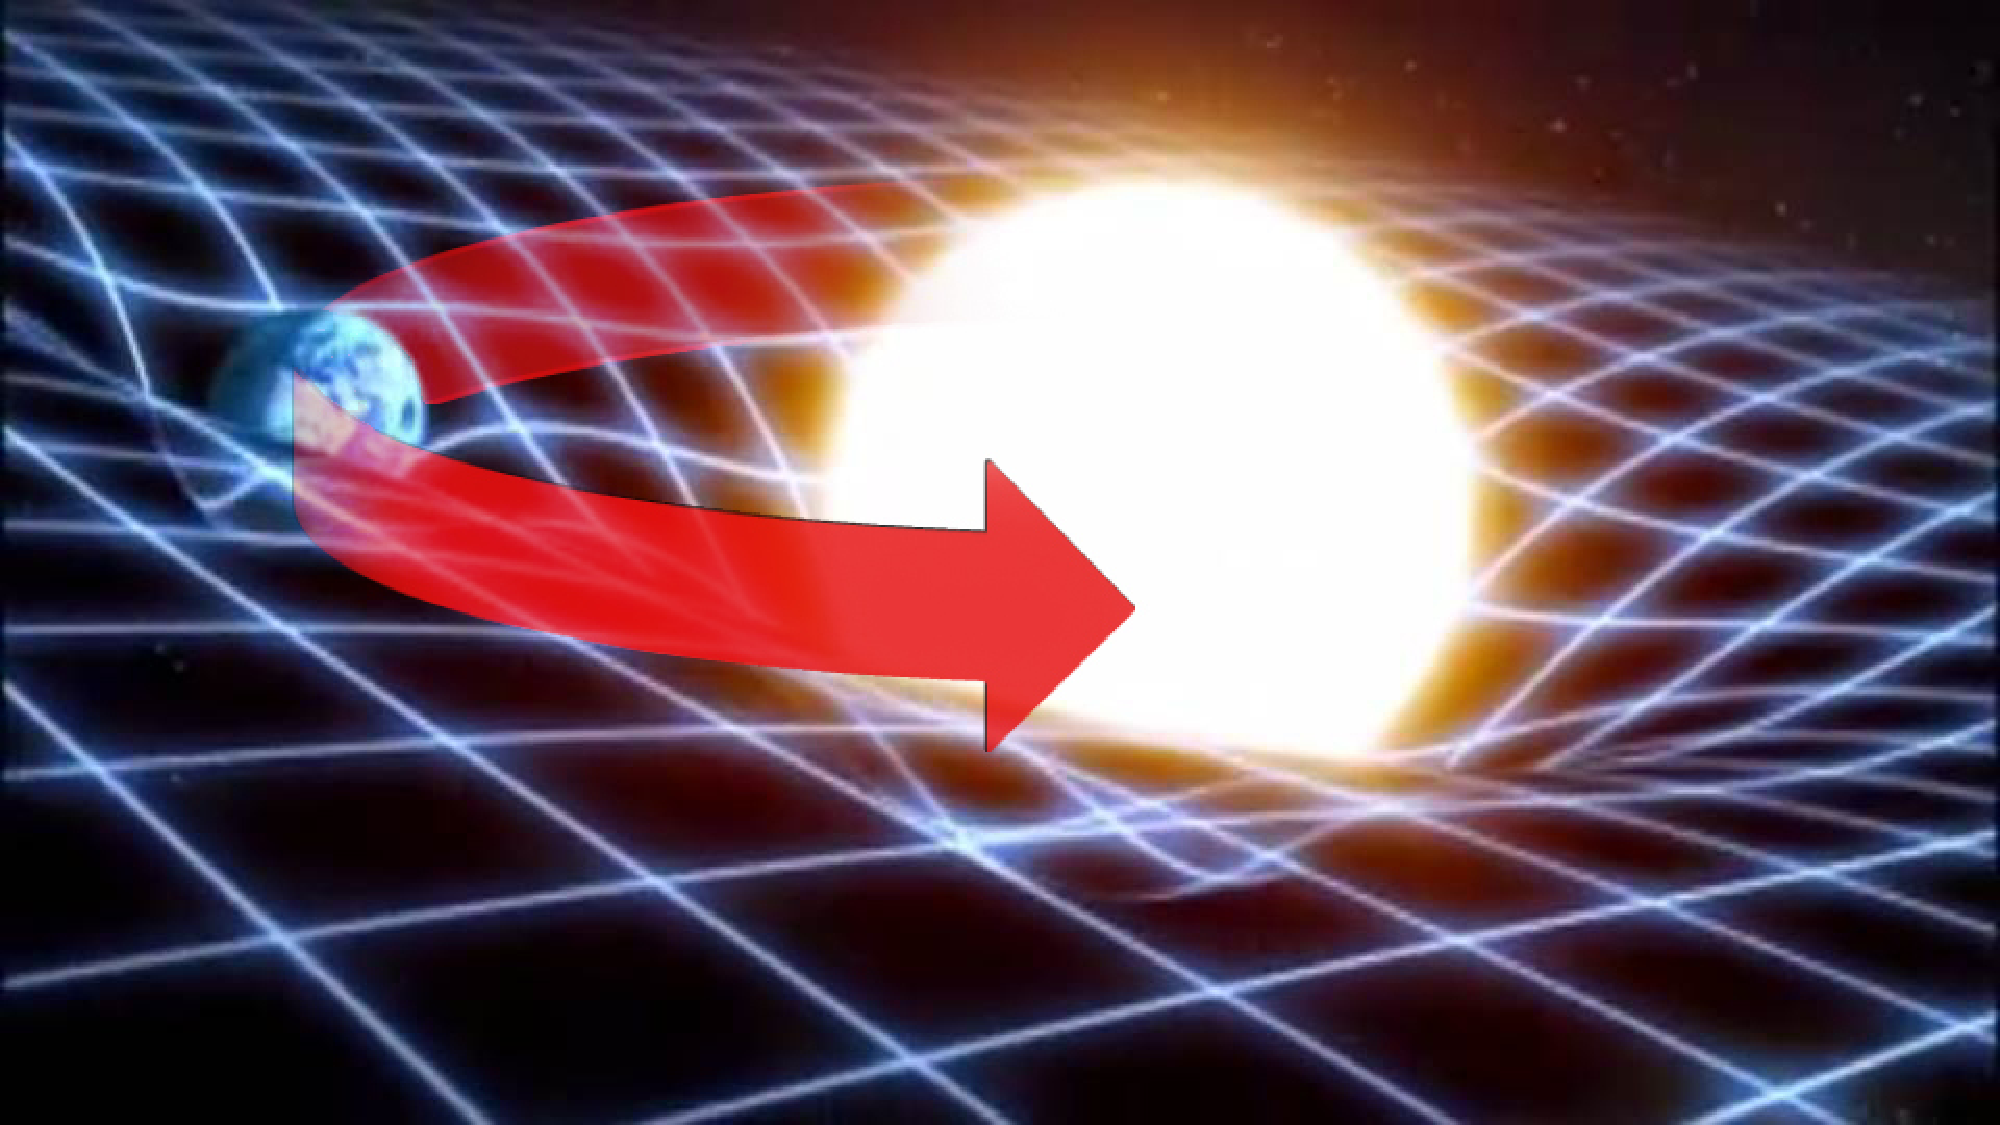
\includegraphics[width=\textwidth,height=0.2\textheight]{spacetime.pdf}
%\end{wrapfigure}
%\end{center}
%\end{figure*}
\end{minipage}
}}
\end{figure*}


There are two things to note in this equation. First, we are using polar coordinates $(r,\phi)$ instead of Cartesian coordinates $(x,y)$. This is a natural choice for a situation with a well defined center. These are not three dimensional coordinates: Symmetry allows us to describe the geometry on \emph{any} plane passing through the center of the central massive body. Given two events with spacetime distance $\Delta s$ as well as the position of the central mass, we have three points in space which define a plane on which we define the polar coordinates. Thus, the $r$ coordinate is a 'distance' from the center, we will later come back to how we measure this distance. The $\phi$ coordinate is the normal $\phi$ angle used in polar coordinates. 

The line element for Lorentz geometry in polar coordinates can similarly be written as
\begin{formbox}
\textbf{Lorentz line element in polar coordinates} 
\[
\Delta s^2=\Delta t^2-\Delta x^2=\Delta t^2-\Delta r^2-r^2\Delta\phi^2.
\]
\end{formbox}

The second thing to note in the equation for the \ss line element is the term $1-2M/r$. Here $M/r$ must be dimensionless since it is added to a number. But we know that mass is measured in kilograms and distances in meters, so how can this term be dimensionless? Actually, there should have been a $G/c^2$ here, $G=6.67\times10^{-11}{\rm\ m^3/kg/s^2}$ being the gravitational constant and $c=3\times 10^8{\rm\ m/s}$ being the speed of light. We have that
\begin{equation}
\label{eq:gc2}
\frac{G}{c^2}=7.42\times10^{-28}{\rm\ m/kg}.
\end{equation}
Since $M/r$ has units $\mathrm{kg}/\mathrm{m}$, $G/c^2$ is clearly the constant which is missing here. We are now used to measure time intervals in units of meters. If we now decide to also measure mass in units of meters, equation (\ref{eq:gc2}) gives us a natural conversion factor.
\begin{formbox}
\[
\frac{M_\mathrm{m}}{M_\mathrm{kg}}=\frac{G}{c^2},
\]
where $M_\mathrm{m}$ is mass measured in meters and $M_\mathrm{kg}$ is mass measured in kg.
\end{formbox}
Thus we have that
\[
1{\rm\ kg}=7.42\times10^{-28}{\rm\ m}.
\]
The equation gives us a conversion formula from kg to m. We see that measuring mass in meters equals setting $G/c^2=1$ everywhere in the formulas. This is equal to what happened when we decided to measure time in meters, we could set $c=1$ everywhere. The reason for measuring mass in meters is pure laziness, it means that we don't need to write this factor all the time when doing calculations. Thus instead of writing $1-2M_\mathrm{kg}G/(rc^2)$ we write $1-2M/r$ where $M$ is now mass measured in meters. All the physics is captured in the last expression, we have just got rid of a constant. From now on, all masses will be measured in units of meters and when we have the final answer we convert to normal units by multiplying or dividing by the necessary factors of $G/c^2$ and $c$ in order to obtain the units that we wish.

\section{The inertial frame}
\label{sect:intertframe}

\begin{Figure}
%\begin{center}
\centering
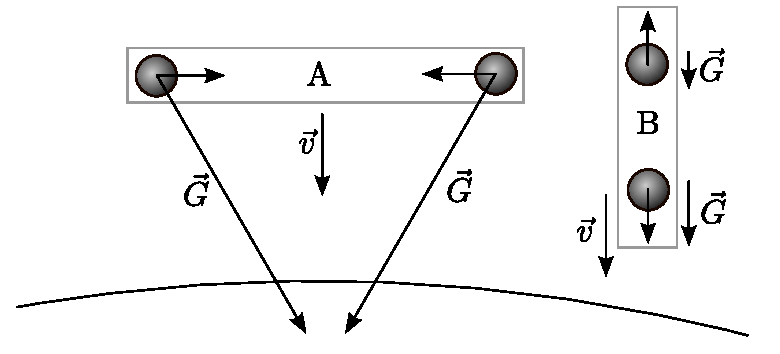
\includegraphics[width=\textwidth]{fig_15-1.pdf}
\captionof{figure}{Two boxes in free fall: If they are large enough in either direction, the objects at rest inside the boxes will start moving. A local inertial frame needs to be small enough in space and time such that this motion cannot be measured. \label{fig:inertial}}
%\end{center}
\end{Figure}


In the lectures on special relativity we defined inertial frames, or free-float frames, to be frames which are not accelerated, frames moving with constant velocity on which no external forces are acting. We can give a more general definition in the following way: To test if the room where you are sitting at the moment is an inertial frame, take an object, leave it at rest with zero velocity. If the object stays at rest with zero velocity, you are in an inertial frame. If you give the object a velocity $v$ and the object continues in a straight line with velocity $v$, you are in an inertial frame. Clearly, a frame (a room) which is not accelerated on which no external forces work is an inertial frame according to this definition. But are there other examples? In general relativity we use the notion of a {\it local internal frame}, i.e.\ limited regions of spacetime which are inertial frames. An example of such a local inertial frame is a space craft in orbit around the Earth. Another example is an elevator for which all cables have broken so that it is freely falling. All freely falling frames can be local inertial frames. How do we know that? If an astronaut in the orbiting space craft takes an object and leaves it with zero velocity, it stays with zero velocity. This is why the astronauts experience weightlessness. If a person in a freely falling elevator takes an object and leaves it at rest, it stays at rest. Also the person in the elevator experiences weightlessness. Thus, they are both, within certain limits, in an inertial frame even though they are both accelerated. Note that an observer standing on the surface of Earth is in a local inertial frame for a very short period of time: If an observer on Earth leaves an object at rest, it will start falling, it will not stay at rest: An observer at the surface of Earth is not in a local inertial frame unless the time interval considered is so short that the effect of the gravitational acceleration is not measurable. The only thing that keeps the observer on the surface of the Earth from being in a local inertial frame is the ground which exerts an upward force on the observer. If suddenly a hole in the ground opens below him and he starts freely falling, he suddenly finds himself in an inertial frame with less strict time limits.




We now need to find out which limitations this inertial frame has. Local means that the inertial frame is limited in space and time, but we need to define these limits. In figure \ref{fig:inertial} we see two falling boxes, box A falling in the horizontal position, box B falling in the vertical position. Since the gravitational acceleration is directed towards the center of the Earth, two objects at rest at either side of box A will start moving towards the center of the box due to the direction of the acceleration. The shorter we make the box, the smaller this motion is. If we make the box so short that we cannot measure the horizontal motion of the objects, we say that the box is a local inertial frame. The same argument goes for time: If we wait long enough, we will eventually observe that the two objects have moved. The inertial frame is limited in time by the time it takes until the motion of the two objects can be measured. Similarly for box B: The object which is closer to the Earth will experience a stronger gravitational force than the object in the other end of the box. Thus, if the box is long enough, an observer in the box will observe the two objects to move away from each other. This is just the normal tidal forces: The gravitational attraction of the moon makes the oceans on either side of the Earth move away from each other: we get high tides. But if the box is small enough, the difference in the gravitational acceleration is so small that the motion of the objects cannot be measured. Again, it is a question of time before a motion will be measured: The local inertial frame is limited in time. We have thus seen that a local inertial frame can be found if we define the frame so small in space and time that the gravitational acceleration within the frame (in space and time) is constant. In these frames, within the limited spatial extent and limited duration in time, an object which is left at rest will remain at rest in that frame. The stronger the gravitational field and the larger the variations in the gravitational field, the smaller in space and time we need to define our local inertial frame. 

We have learned from special relativity that an inertial frame has Lorentz geometry. Within the local inertial frame, spacetime intervals are measured according to $\Delta s^2=\Delta t^2-\Delta x^2$ and the laws of special relativity are all valid within the limits of this frame. In general relativity, we can view spacetime around a massive object as being an infinite set of local inertial frames. When performing experiments within these limited frames, special relativity is all we need. When studying events taking place so far apart in space and time that they do not fit into one such local inertial frame, general relativity is needed. This is why only special relativity is needed for particle physicists making experiments in particle accelerators. The particle collisions take place in such a short time that the gravitational acceleration may be neglected: They take place in a local inertial frame.

We will now call spacetime where Lorentz geometry is valid {\it flat spacetime}. This is because Lorentz geometry is similar to Euclidean geometry on a flat surface (except for a minus sign). We know that a curved surface, like the surface of the sphere, has spherical geometry not Euclidean geometry. In the same way, \ss geometry represents {\it curved spacetime}, the rules of Lorentz geometry are not valid and \ss geometry needs to be used. We say that the presence of matter curves spacetime. Far away from all massive bodies, spacetime is flat and special relativity is valid. 

We can take the analogy even further: Since the surface of a sphere has spherical and not Euclidean geometry, the rules of Euclidean geometry may not be used. But if we focus on a very small part of the surface of a sphere, the surface looks almost flat and Euclidean geometry is a very good approximation. The surface of the Earth is curved and therefore has spherical geometry, but since a garden is very small compared to the full surface of the Earth, the surface of the Earth appears to us to have flat geometry within the garden. We use Euclidean geometry when measuring the area of the garden. The same is the case for the curved space: Since spacetime is curved around a massive object, we need to use \ss geometry. But if we only study events which are within a small area in spacetime, spacetime looks flat and Lorentz geometry (the local inertial frame) is a good approximation.

\section{Three observers}
\label{sect:observers}

In the lectures on general relativity we will use three observers, {\it the far-away observer}, {\it the shell observer} and {\it the freely falling observer}. We will also assume that the central massive body is a black hole. A black hole is the simplest possible macroscopic object in universe: it can be described by three parameters, mass, angular momentum and charge. Any black holes which have the same values for these three parameters are identical in the same way as two electrons are identical. A black hole is a region in space where the gravitational acceleration is so high that not even light can escape from it. A black hole can arise for instance when a massive star is dying: A star is balanced by two forces, the forces of gravity (which we no longer call forces) trying to pull the star together and the gas/radiation pressure trying to make the star expand. When all fuel in the stellar core is exhausted, the forces of pressure are not strong enough to withstand the forces of gravity and the star collapses. No forces can stop the star from shrinking to an infinitely small point. The gravitational acceleration just outside this point is so large that even light that tries to escape will fall back. The escape velocity is larger than the speed of light. This is a black hole. Note that the \ss line element becomes singular at $r=2M$. This radius is called the {\it \ss radius} or {\it the horizon}. This is the 'point of no return', any object (or light) which comes inside this horizon cannot get out. At any point before the horizon a spaceship with strong engines could still escape. But after it has entered, no information can be transferred out of the horizon.

The {\it far-away observer} is situated in a region far from the central black hole where spacetime is flat. He does not observe any events directly, but gets information about time and position of events from clocks situated everywhere around the black hole. {\it The shell observers} live on the surface of shells constructed around the black hole. Also a spaceship which uses its engines to stay at rest at a fixed radius $r$ could serve as a shell observer. The shell observers experience the gravitational attraction. When they leave an object at rest it falls to the surface of the shell. 

There is one more observer which we already discussed in the previous section. This is the {\it freely falling observer}. The freely falling observer carries with him a wristwatch and registers the position and personal wristwatch time of events. The freely falling observer is living in a local inertial frame with flat spacetime. Thus for events taking place within short time intervals and short distances in space, the freely falling observer uses Lorentz geometry to make calculations.

\section{The time and position coordinates for the three observers}
\label{sect:coordinates}

Each of the observers have their own set of measures of time and space. The far away observer uses \ss coordinates $(r,t)$ and shell observers use shell coordinates $(r_\sh,t_\sh)$. For the freely falling observers, we will be viewing all events from the origin in his frame of reference (and we will therefore not need a position coordinate since it will always be zero) using his wristwatch time which will then always be the proper time $\tau$. We will now discuss these different coordinate systems and how they are defined.


When the shell observer wants to measure his position $r$ from the center of the black hole, he runs into problems: When he tries to lower a meter stick down to the center of the hole to measure $r$, the stick just disappears behind the horizon. He needs to find other means to measure his radial position. What he does is to measure the circumference of his shell. In Euclidean geometry, we know that the circumference of a circle is just $2\pi r$. So the shell observer measures the circumference of the shell and divides by $2\pi$ to obtain his coordinate $r$. In a non-Euclidean geometry, the radius measured this way does not correspond to the radius measured inwards. We \emph{define} the {\it \ss coordinate} $r$ in this way. 
\[
r=\frac{\mathrm{circumference}}{2\pi}
\]

The $r$ in the expression for the \ss line element is the \ss coordinate $r$. Now the shell observers at shell $r$ lower a stick to the shell observers at shell $r'$. The length of the stick is $\Delta r_\sh$. They compare this to the difference in \ss coordinate $r-r'$ and find that $\Delta r_\sh\ne\Delta r=r-r'$. This is what we anticipated, in Euclidean geometry these need to be equal, in \ss geometry they are not. We have obtained a second way to measure the radial distances between shells using shell distances $\Delta r_\sh$ (note that since the absolute shell coordinate $r_\sh$ cannot be measured it is meaningless, only relative shell coordinate differences $\Delta r_\sh$ between shells can be measured (did you understand why?)).

We have obtained two different measures of radial distances, 
\begin{itemize}
\item the \ss coordinate $r$ defined by the circumference of the shell. The far-away observer uses \ss coordinates to measure distances.
\item the shell distances $\Delta r_\sh$ found by physical measurements between shells.This is the distance which the shell observers can measure directly with meter sticks and is therefore the most natural measure for these observers.
\end{itemize}

What about time coordinates? Again we have two meaures of time,
\begin{itemize}
\item The far-away observer uses {\it far-away time} $t$ to measure time. This is the time $t$ entering in the \ss line element. Far away time for an event is measured on a clock which has been synchronized with the clock of the far-away observer and which is located at the same location as the event (we will later describe how events can be timed which such clocks in practice).

\item The shell observer uses local shell time $t_\sh$: it is simply the wristwatch time of the shell observer, the time measured on a clock at rest at the specified shell. Note that shell observers at different shells may measure different times intervals $\Delta t_\sh$ and distances $\Delta r_\sh$ between two events depending on which shell they live on. Shell coordinates are local coordinates. 
\end{itemize}

In order to relate time and space coordinates in the different frames we will now (as we did in special relativity) use the invariance of the space time interval (or line element) $\Delta s$. First we will find a relation between the more abstract far away-time $t$ and the locally measurable shell time $t_\sh$. The shell time is the wristwatch time, or proper time $\tau$ of the shell observers. We will use two events A and B which are two ticks on the clock of a shell observer. The shell observers are at rest at shell $r$, so , $\Delta r_{AB}=0$ and $\Delta \phi_{AB}=0$. Inserting this into the \ss line element (equation \ref{eq:ss}) using that $\Delta s_{AB}=\Delta\tau_{AB}=\Delta t_\sh$ (the time period between A and B measured on shell clocks is by definition the same as the proper time period between A and B which we have learned is always equal to the invariant four dimensional line element between these events) we get
\begin{formbox}
\textbf{Shell time}
\begin{equation}
\label{eq:tt}
\Delta t_\sh=\sqrt{\sst} \Delta t.
\end{equation}
\end{formbox}
(Are you sure you see how this expression comes about?) For shell observers outside the horizon ($r>2M$), the local time goes slower by a factor $\sqrt{\sst}$ with respect to the far-away time. We also see that the smaller the distance $r$ from the center, the slower the shell clock with respect to the far-away time. Thus, the further down we live in a gravitational field, the slower the clocks run. This has consequences for people living on Earth: Our clocks tick slower than the clocks in satellites in orbit around Earth. At the end of this lecture, we will look closer at this fact.

\begin{Figure}
%\begin{center}
\centering
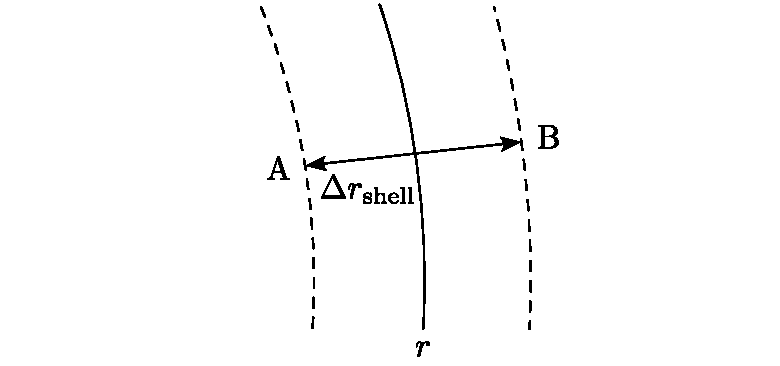
\includegraphics[width=\textwidth]{fig_15-2.pdf}
\captionof{figure}{The shell observer at shell $r$  measure the proper lenght of a stick by two simultaneous events A and B on either side of the stick. \label{fig:stick}}
%\end{center}
\end{Figure}

We have now found a relation between time intervals measured on shell clocks and time intervals measured on clocks synchronized with far-away clocks. How is the relation between distances measured with \ss coordinates and distances measured directly by shell observers? We can measure the length of a stick as the spatial distance between two events taking place at the same time at either end of the stick (see figure \ref{fig:stick}). For events taking place within short time intervals and short spatial extensions, the shell observer sees flat spacetime and can therefore use Lorentz geometry: \mbox{$\Delta s_\sh^2=\Delta t_\sh^2-\Delta r_\sh^2$} (we will look at a stick which is aligned with the radial direction, the events therefore take place at the same $\phi$ coordinate so $\Delta\phi=0$). The far-away observer always needs to use the \ss line element (equation \ref{eq:ss}) instead of the Lorentz line element. Using invariance of the line element we have for two events A and B \mbox{($\Delta s_\sh(AB)=\Delta s(AB)$)} taking place simultaneously on either side of the stick
\[
\Delta t_\sh^2-\Delta r_\sh^2=\sst \Delta t^2-\frac{\Delta r^2}{\sst},
\]
where we have set $\Delta\phi=0$. Check that you understand how to arrive at this expression. Now, we measure the length $\Delta r$ of a stick in the radial direction by measuring the distance between the two simultaneous events A and B taking place at either end of the stick at spatial distance $\Delta r$. Since events which are simultaneous for shell observers at a given shell $r$ also are simultaneous for the far-away observer (equation \ref{eq:tt}), $\Delta t_\sh=\Delta t=0$. Inserting this, we get
\begin{formbox}
\begin{equation}
\label{eq:rr}
\Delta r_\sh=\frac{\Delta r}{\sqrt{\sst}}.
\end{equation}
\end{formbox}
for short distances $\Delta r$ close to the shell.
Thus, radial distances measured by the shell observers, lowering meter sticks from one shell to the other is always larger than the radial distances found by taking the difference between the \ss coordinate distances. What about a stick which is perpendicular to the radial direction? In this case, the observers will agree on the length of this stick, check that you can deduce this in the same manner as we deduced the relation for the radial stick.

There is a practical problem in all this: We said that the far-away time was measured by clocks located at the position of events (which can take place close to the central black hole) but which are synchronized with the far-away clocks. How can we synchronize clocks which are located deep in the gravitational field and which therefore run slower than the far-away clock? Let's imagine the clocks measuring far-away-time to be positioned at different shells around the black hole. The shell observers design the clocks such that they run faster by a factor $\sqrt{\sst}$. To synchronize all these clocks, the far-away observer sends a light signal to all the other clocks at the moment when he sets his clock to $t=0$. The shell observers know the distance from the far-away observer to the far-away-time clocks and thus know the time $t$ it took for the light signal to reach their clock. They had thus already set the clock to this time $t$ and made a mechanism such that it started to run at the moment when the light signal arrived. In this way, all far-away-time clocks situated at different positions around the black hole are synchronized. 

Another practical question: How does the far-away observer know the time and position of events. Each time an event happens close to one of the far-away-clocks close to the black hole, it sends a signal to the far-away observer telling the time and position this clock registered for the event. In this way, the far-away observer does not need to take into account the time it takes for the signal from the clock to arrive, the signal itself contains information with the correct far-away-time for the event recorded on the clock positioned at the same location where the event took place.


In the following we will describe events either as they are seen by the far-away observer using global \ss coordinates $(r,t)$, by the shell observer using local coordinates $(r_\sh,t_\sh)$ or the freely falling observer also using local coordinates. Before proceeding, make a drawing of all these observers, their coordinates and the relation between these different coordinates.

\section{The principle of maximum aging revisited}
\label{sect:maxaging}

In the lectures on special relativity we learned that the principle of maximum aging tells objects in free float to move along paths in spacetime which give the longest possible wristwatch time $\tau$ which corresponds to the longest possible spacetime interval $s$. We also used that for Lorentz geometry, the longest (in terms of $s$ or $\tau$) path between two points is the straight line, i.e.\ the path with constant velocity. We never proved the latter result properly. We will do this now, first for Lorentz geometry and then we will use the same approach to find the result for \ss geometry.

\subsection{Returning for a moment to special relativity: deducing Netwon's first law}

We will now show that the principle of maximum aging leads to Newton's first law when using Lorentz geometry.

\begin{Figure}
%\begin{center}
\centering
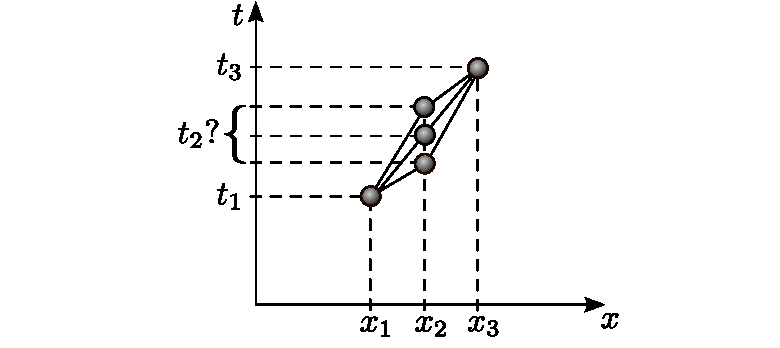
\includegraphics[width=\textwidth]{fig_15-3.pdf}
\captionof{figure}{The motion of a particle in free float in Lorentz geometry. Points $x_1$, $x_2$, $x_3$ as well as the times $t_1$ and $t_3$ are fixed. For a particle at free float, at what time $t_2$ will it pass $x_2$? Which of the possible spacetime paths in the figure does the particle take? We use the principle of maximal aging to show that in Lorentz geometry, the particle follows the straight spacetime path. \label{fig:123}}
%\end{center}
\end{Figure}


Look at figure \ref{fig:123}. We see the worldline of a particle going from position $x_1$ at time $t_1$ to position $x_3$ at time $t_3$ passing through position $x_2$ at time $t_2$. Say that the points $x_1$, $x_2$ and $x_3$ are fixed and known positions. We also say that the total time interval $t_{13}$ it takes the object to go from $x_1$ to $x_3$ is fixed and known. What we do not know is the time interval $t_{12}$ it takes the particle to go from point $x_1$ to point $x_2$. Remember that we do not know that the object will move with constant velocity, this is what we want to show. Thus we leave open the possibility that the particle will have a different speed between $x_1$ and $x_2$ than between $x_2$ and $x_3$. The time $t_2$ can be at any possible point between $t_1$ and $t_3$. In figure \ref{fig:123} we show some possible spacetime paths that the object could take. We now assume that the distances $x_{12}$ and $x_{23}$ are very short, so short that the object can be assumed to move with constant velocity between these two points, i.e.\ that the object is in a local inertial frame between $x_1$ and $x_2$ and in a (possibly different) intertial frame between $x_2$ and $x_3$. Therefore, the time intervals $t_{12}$ and $t_{23}$ to travel these two short paths also need to be short.

The total wristwatch time $\tau$ it takes the particle to move from $x_1$ to $x_3$ is
\begin{equation}
\label{eq:maxag}
\tau_{13}=\tau_{12}+\tau_{23}=\sqrt{t_{12}^2-x_{12}^2}+\sqrt{t_{23}^2-x_{23}^2},
\end{equation}
where we used that $\Delta\tau=\Delta s=\sqrt{\Delta t^2-\Delta x^2}$ for Lorentz geometry. According to the principle of maximal aging, we need to find the path, i.e.\ the $t_{2}$, which maximizes the total wristwatch time $\tau_{13}$. We do this by setting the derivative of $\tau_{13}$ with respect to the free parameter $t_{2}$ equal to zero, i.e.\ you look for the maximum point of the function $\tau_{13}(t_{2})$:
\[
\frac{d\tau_{13}}{dt_{2}}=\frac{t_{12}}{\sqrt{t_{12}^2-x_{12}^2}}\frac{dt_{12}}{dt_{2}}.+\frac{t_{23}}{\sqrt{t_{23}^2-x_{23}^2}}\frac{dt_{23}}{dt_{2}}.
\]
Since $t_{12}=t_{2}-t_{1}$ we have that $dt_{12}/dt_{2}=1$ (remember that $t_{1}$ is a fixed constant) and similarly for $t_{23}$. Thus we have
\[
\frac{t_{12}}{\sqrt{t_{12}^2-x_{12}^2}}-\frac{t_{23}}{\sqrt{t_{23}^2-x_{23}^2}}=0
\]
or written in terms of $\tau_{12}$ and $\tau_{23}$ we have
\[
\frac{t_{12}}{\tau_{12}}=\frac{t_{23}}{\tau_{23}}.
\]
Check that you understood every step in the deduction so far! This is only for three points $x_1$, $x_2$ and $x_3$ along the worldline of a particle. If we continue to break up the worldline in small local inertial frames at points $x_4$, $x_5$, etc. we can do the same analysis between any three adjacent points along the curve. The result is that
\[
\frac{dt}{d\tau}=\mathrm{constant},
\]
where I have written $dt$ instead of $t_{12}$ or $t_{23}$ and $d\tau$ instead of $\tau_{12}$ or $\tau_{23}$. Remember that we assumed these time intervals to be very short. In this final expression we have taken the limit in which these time intervals are infinitesimally short. We also remember (do you?) from special relativity that
\[
\frac{dt}{d\tau}=\frac{1}{\sqrt{1-v^2}}=\gamma.
\]
So the principle of maximal aging has given us that $\gamma=\mathrm{constant}$ along a worldline. But $\gamma$ only contains the velocity $v$ of the object so it follows that $v=\mathrm{constant}$. In Lorentz geometry, a free-float object will follow the spacetime path for which the velocity is constant. We can write this in a different way. In special relativity we had that
\[
E=\gamma m
\]
so we can write $\gamma=E/m$ from which follows that
\[
\gamma=\frac{E}{m}=\mathrm{constant}.
\]
We have just deduced that energy is conserved, or more precisely energy per mass $E/m$ is conserved. In the lectures on special relativity we learned that experiments tell us that the relativistic energy $E=\gamma m$ is conserved and not Newtonian energy. Here we found that the principle of maximal aging tells us that there is a quantity which is conserved along the motion of a particle. This quantity is the same as the quantity we call relativistic energy. 

\begin{Figure}
%\begin{center}
\centering
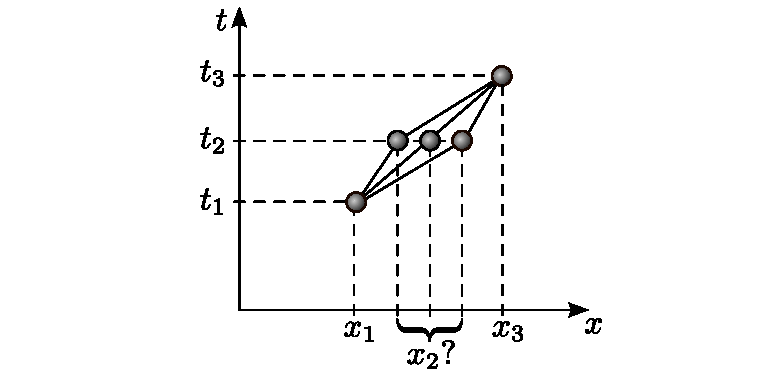
\includegraphics[width=\textwidth]{fig_15-4.pdf}
\captionof{figure}{The motion of a particle in free float in Lorentz geometry. Points $x_1$, $x_3$ as well as the times $t_1$, $t_2$ and $t_3$ are fixed. For a particle in free float, which position $x_2$ will it pass at time $t_2$? Which of the possible spacetime paths in the figure does the particle take? We use the principle of maximal aging to show that in Lorentz geometry, the particle follows the straight spacetime path. \label{fig:p123}}
%\end{center}
\end{Figure}


Is it possible that the principle of maximal aging can give us something more? We will now repeat the above calculations, but now we fix $t_{1}$, $t_{2}$ and $t_{3}$. All times are fixed. We also fix $x_1$ and $x_3$, but leave $x_2$ free. The situation is shown in figure \ref{fig:p123}. Now the question is 'which point $x_2$ will the object pass through?'. We need to take the derivative of expression (\ref{eq:maxag}) with respect to $x_{2}$ which is a free parameter.
\[
\frac{d\tau_{13}}{dx_{2}}=\frac{-x_{12}}{\sqrt{t_{12}^2-x_{12}^2}}\frac{dx_{23}}{dx_{12}}.-\frac{x_{2}}{\sqrt{t_{12}^2-x_{12}^2}}\frac{dx_{23}}{dx_{2}}.
\]
Again $x_{12}=x_{2}-x_{1}$ so that $dx_{12}/dx_{2}=1$ (and similarly for $x_{23}$) and we have
\[
\frac{x_{12}}{\tau_{12}}=\frac{x_{23}}{\tau_{23}},
\]
we have found another constant of motion
\[
\frac{dx}{d\tau}=\mathrm{constant}
\]
But we can write this as
\[
\frac{dx}{d\tau}=\frac{dx}{dt}\frac{dt}{d\tau}=v\gamma.
\]
We have that
\[
v\gamma=\mathrm{constant}=\frac{p}{m}.
\]
(Go through this deduction in detail yourself and make sure you understand every step). We remember that $p=m\gamma v$, so the principle of maximal aging has given us the law of momentum conservation, or actually the law of conservation of momentum per mass $p/m$. We have seen that the principle of maximal aging seems to be more fundamental than the principles of energy and momentum conservation. It is sufficient to assume the principle of maximal aging. From that we can deduce the expressions for energy and momentum and also that these need to be conserved quantities.


\subsection{Returning to general relativity: deducing and generalizing Newton's law of gravitation}

\begin{Figure}
%\begin{center}
\centering
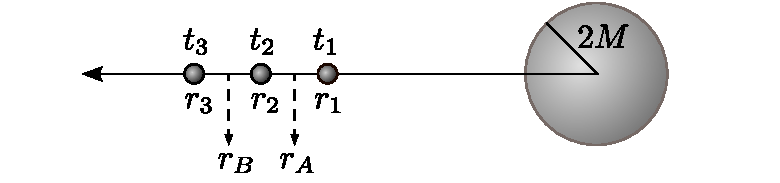
\includegraphics[width=\textwidth]{fig_15-5.pdf}
\captionof{figure}{The motion of a particle in free float in \ss geometry. Points $r_1$, $r_2$, $r_3$ as well as the times $t_1$ and $t_3$ are fixed. For a particle in free float, at what time $t_2$ will it pass through $r_2$? We assume that the distances $r_2-r_1$ and $r_3-r_2$ are so small that we can assume the radial distance to be $r=r_A$ always in the former interval and $r=r_B$ always in the latter interval. \label{fig:gr123}}
%\end{center}
\end{Figure}

\begin{Figure}
%\begin{center}
\centering
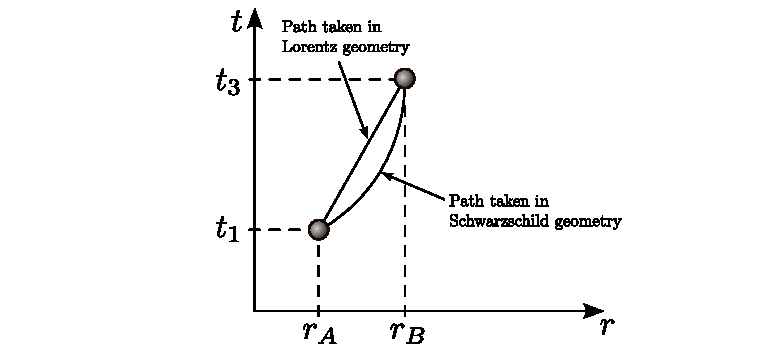
\includegraphics[width=\textwidth]{fig_15-6.pdf}
\captionof{figure}{The motion of a particle in free float in \ss geometry. Which spacetime path will the particle take between points A and B? \label{fig:ab}}
%\end{center}
\end{Figure}

Now, what about general relativity? We will see how the principle of maximal aging tells a particle to move in \ss spacetime. Look at figure \ref{fig:gr123}. A particle travels from radius $r_1$ at time $t_1$ to radius $r_3$ at point $t_3$ passing through point $r_2$ at time $t_2$. We fix $r_1$, $r_2$ and $r_3$. We also fix the start and end times $t_1$ and $t_3$. We leave $t_2$ free. We will find at which time $t_2$ the particle passes through point $r_2$. Again we write the total proper time for the object from $r_1$ to $r_3$ as (using the \ss line element, equation \ref{eq:ss}, for $\Delta\tau$)
\begin{align*}
&\tau_{13}=\tau_{12}+\tau_{23}=\sqrt{\left(1-\frac{2M}{r_A}\right)t_{12}^2-\frac{r_{12}^2}{\left(1-\frac{2M}{r_A}\right)}} \\
& \qquad +\sqrt{\left(1-\frac{2M}{r_B}\right)t_{23}^2-\frac{r_{23}^2}{\left(1-\frac{2M}{r_B}\right)}},
\end{align*}
where $r_A$ is the radius halfway between $r_1$ and $r_2$. We assume that $r_{12}$ is so small that we can use the radius $r_A$ for the full interval. In the same way, $r_B$ is the radius halfway between $r_2$ and $r_3$ which we count as valid for the full interval $r_{23}$. Following the procedure above, we will now maximize the total proper time $\tau_{13}$ with respect to the free parameter $t_{2}$. We get
\[
\frac{d\tau_{13}}{dt_{2}}=\frac{\left(1-\frac{2M}{r_A}\right)t_{12}}{\tau_{12}}\frac{dt_{12}}{dt_{2}}+\frac{\left(1-\frac{2M}{r_B}\right)t_{23}}{\tau_{23}}\frac{dt_{23}}{dt_{2}}.
\]
As above, $t_{12}=t_{2}-t_{1}$ giving $dt_{12}/dt_{2}=1$ (and similarly for $t_{23}$). Thus we have that
\[
\frac{\left(1-\frac{2M}{r_A}\right)t_{12}}{\tau_{12}}=\frac{\left(1-\frac{2M}{r_B}\right)t_{23}}{\tau_{23}}.
\]
We find that
\begin{equation}
\label{eq:gene}
\sst\frac{dt}{d\tau}=\mathrm{constant},
\end{equation}
where again we have taken the limit where $t_{12}$, $t_{23}$, $\tau_{12}$ and $\tau_{13}$ are so small that they can be expressed as infinitesimally small periods of time $dt$ and $d\tau$. In the case with Lorentz geometry we used this constant of motion to find that the velocity had to be constant along the worldline of a freely floating particle. Now we want to investigate how this constant of motion tells us how a freely floating particle moves in \ss spacetime. First we need to find an expression for $dt/d\tau$. In special relativity we related this to the velocity of the particle using $dt/d\tau=\gamma$, but this was deduced using the line element of Lorentz geometry. Here we want to relate this to the local velocity that a shell observer at a given radius observes. The locally measured shell velocity as an object passes by a given shell is given by
\[
v_\sh=\frac{dr_\sh}{dt_\sh}
\]
We now use equation \ref{eq:tt} (the equation connecting far-away-time and shell time, remember?) to write the constant of motion (equation \ref{eq:gene}) as
\begin{align*}
&\sst\frac{\sst^{-1/2}dt_\sh}{d\tau}\\
&=\sst^{1/2}\frac{dt_\sh}{d\tau}\\
&=\sst^{1/2}\gamma_\sh\\
&=\sst^{1/2}\frac{1}{\sqrt{1-v_\sh^2}}=\mathrm{constant}.
\end{align*}
In the last transition we used the fact that the shell observer lives in a local inertial frame for a very short time. The shell observer makes the velocity measurement so fast that the gravitational acceleration could not be noticed and he could use special relativity assuming flat spacetime. So using his local time $t_\sh$, the relation $dt_\sh/d\tau=\gamma_\sh$ from special relativity is valid. We have thus found a constant of motion:
\[
\sst^{1/2}\frac{1}{\sqrt{1-v_\sh^2}}=\mathrm{constant}.
\]

Consider a particle moving from radius $r_A$ to a higher radius $r_B$ (see figure \ref{fig:ab}). This time, the distance between points A and B does not need to be small. As the object moves past shell $r_A$, the shell observers at this shell measure the local velocity $v_A$. As the object moves past shell $r_B$, the shell observers at this shell measure the local velocity $v_B$. Equating this constant of motion at the two positions A and B we find
\[
\left(1-\frac{2M}{r_A}\right)^{1/2}\frac{1}{\sqrt{1-v_A^2}}=\left(1-\frac{2M}{r_B}\right)^{1/2}\frac{1}{\sqrt{1-v_B^2}}.
\]
Squaring and reorganizing we find
\[
(1-v_B^2)\left(1-\frac{2M}{r_A}\right)=(1-v_A^2)\left(1-\frac{2M}{r_B}\right).
\]
We already see from this equation that if $r_B>r_A$ then $v_B<v_A$ (check!). Thus if the object is moving away from the central mass, the velocity is decreasing. If we have $r_B<r_A$ we see that the opposite is true: If the object is moving towards the central mass, the velocity is increasing. So the principle of maximum aging applied in \ss geometry gives a very different result than in Lorentz geometry. In Lorentz geometry we found that the velocity of a freely floating particle is constant. In \ss spacetime we find that the freely floating particle accelerates towards the central mass: If it moved outward it slows down, if it moved inwards it accelerates. This is just what we normally consider the 'force of gravity'. We see that here we have not included any forces at all: We have just said that the central mass curves spacetime giving it \ss geometry. By applying the principle of maximal aging, that an object moving through spacetime takes the path with longest possible wristwatch time $\tau$, we found that the object needs to take a path in spacetime such that it accelerates towards the central mass. We see how geometry of spacetime gives rise to the 'force of gravity'. But in general relativity we do not need to introduce a force, we just need one simple principle: The principle of maximal aging.

We will now check if the acceleration we obtain in the limit of large radius $r$ and low velocities $v_\sh$ is equal to the Newtonian expression. We now call the constant of motion $K$ giving
\[
\sst\frac{1}{1-v_\sh^2}=K.
\]
Reorganizing this we have
\begin{equation}
\label{eq:vshell}
v_\sh=\sqrt{1-\frac{1}{K}\sst}
\end{equation}
We want to find the acceleration
\[
g_\sh=\frac{dv_\sh}{dt_\sh}
\]
that a shell observer measures. Taking the derivative of equation \ref{eq:vshell} we get (check!)
\[
\frac{dv_\sh}{dt_\sh}=\frac{1}{2v_\sh}\frac{2M}{K}\left(-\frac{1}{r^2}\right)\frac{dr}{dt_\sh}.
\]
Using equation \ref{eq:rr} and that $v_\sh=dr_\sh/dt_\sh$ we obtain
\[
g_\sh\propto \sqrt{\sst}\frac{M}{r^2}
\]
Newton's law of gravitation is not valid close to the \ss horizon, so to take the Newtonian limit we need to consider this expressions for $r\gg2M$. In this limit the expression reduces to
\[
g_\sh\propto\frac{M}{r^2},
\]
exactly the Newtonian expression for the gravitational acceleration. We find that far away from the \ss radius, general relativity reduces to Newton's law of gravitation. We can now return to figure \ref{fig:ab} and look at the path marked \ss path. This is the spacetime path between A and B that a freely floating object needs to take in order to get the longest proper time $\tau$. Looking at the slope of this path, we see that the object changes velocity during its trip from A to B. This is in sharp contrast to the results from special relativity with Lorenzt geometry where the path which gives longest possible proper time is the straight line with constant velocity.

We will now return to our constant of motion
\begin{equation}
\label{eq:constant}
\sst^{1/2}\frac{1}{\sqrt{1-v_\sh^2}}=\mathrm{constant}
\end{equation}
In special relativity we found that a constant of motion which we obtain in the same manner was just the energy per mass. We will now go to the Newtonian limit to see if the same is the case for \ss spacetime. We will use two Taylor expansions,
\begin{align*}
\sqrt{1-x}&\approx 1-\frac{1}{2}x+...\\
\frac{1}{\sqrt{1-x^2}}&\approx 1+\frac{1}{2}x^2,
\end{align*}
both taken in the limit of $x\ll1$. In the Newtonian limit we have that $2M/r\ll1$ and $v\ll1$. Applying this to equation (\ref{eq:constant}) we have
\[
\left(1-\frac{M}{r}\right)\left(1+\frac{1}{2}v^2\right)\approx 1+\frac{1}{2}v^2-\frac{M}{r}=\mathrm{constant}
\]
In the last expression we used that since both $2M/r$ and $v$ are very small, the product of these small quantities is even smaller than the remaining terms and could therefore be omitted. Compare this to the Newtonian expression for the energy of a particle in a gravitational field
\[
E=\frac{1}{2}mv^2-\frac{Mm}{r}.
\]
We see again that the constant of motion was just energy per mass $E/m$ where the expression now tells us how the gravitational potential looks like (have you noticed this: you have actually derived why the form of the Newtonian gravitational potential is the way it is). Note the additional term in the relativistic expression which is just the rest energy $m$. Again the principle of maximal aging has given us that energy is conserved and it has given us the relativistic expression for energy in a gravitational field.
\begin{formbox}
\textbf{Relativistic energy in a gravitational field}
\[
\frac{E}{m}=\sst\frac{dt}{d\tau} = {\rm constant}.
\]
\end{formbox}
We also found that this expression for the energy equals the Newtonian expression for distances far from the \ss radius.

In the exercises you will use the principle of maximum aging to find that angular momentum per mass is conserved in \ss spacetime and that the expression for angular momentum per mass in \ss spacetime is
\begin{formbox}
\textbf{Angular momentum per mass in \ss spacetime}
\[
\frac{L}{m}=r^2\frac{d\phi}{d\tau}=\gamma_\sh r v_\phi=\mathrm{constant}.
\]
\end{formbox}





\section{Freely falling}
\label{sect:falling}

Armed with the expression for the conserved energy and angular momentum we will now start to look at motion around the black hole. First, we will leave an object at rest at a large distance from the central mass. We leave the object with velocity zero $v=0$ at a distance so large that we can let $r\rightarrow\infty$. The energy per mass of the particle is then only the rest energy of the particle, $E=m$.
\[
\frac{E}{m}=\sst\frac{dt}{d\tau}=1
\]
In problem \refproblem{prob:falling} you will use this fact to show that the velocity of the object as it falls towards the central mass as seen by the far away observer is given by
\begin{equation}
\label{eq:v}
v=-\sst\sqrt{\frac{2M}{r}}.
\end{equation}
At large distance $r\rightarrow\infty$ the velocity goes to zero as expected. What happens when the object approaches the black hole? For large distances the factor $\sqrt{2M/r}$ is dominating. This factor increases with decreasing $r$, so the velocity increases just as expected. When we approach the \ss radius, the first factor $\sst$ starts dominating the behaviour of $v$ as the last factor now goes to one. In this case, the velocity is decreasing when $r$ is decreasing. At the horizon the velocity reaches exactly zero. What we see is plotted in figure \ref{fig:falling}. When the object starts falling the velocity increases until a point where it starts decreasing. At the horizon the object stops. This result was obtained using \ss coordinates. Thus, this is the result that the far-away observer sees. This means that if we let a spaceship fall into a black hole, we, as far-away observers, would see the spaceship stopping at the horizon and it would stay there for ever. Remember also that time is going slower closer to the horizon,
\[
\Delta t_\sh=\sqrt{\sst}\Delta t
\]
At the horizon $r\rightarrow 2M$, we observe that time stops. Thus, looking at the spaceship we would observe the persons in the spaceship to freeze at the horizon. Everything stops. In the exercises you will show that light from a central mass is red shifted. Thus we will also see a strongly redshifted light from the spaceship. Using the expression from the exercises you will see that light arriving from the horizon is infinitely red shifted. Thus you will not see any light from the horizon. You will only see the spaceship just before it reaches the horizon and then only as radio waves with a large wavelength (see problem \refproblem{prob:rdoppler}).

\begin{Figure}
%\begin{center}
\centering
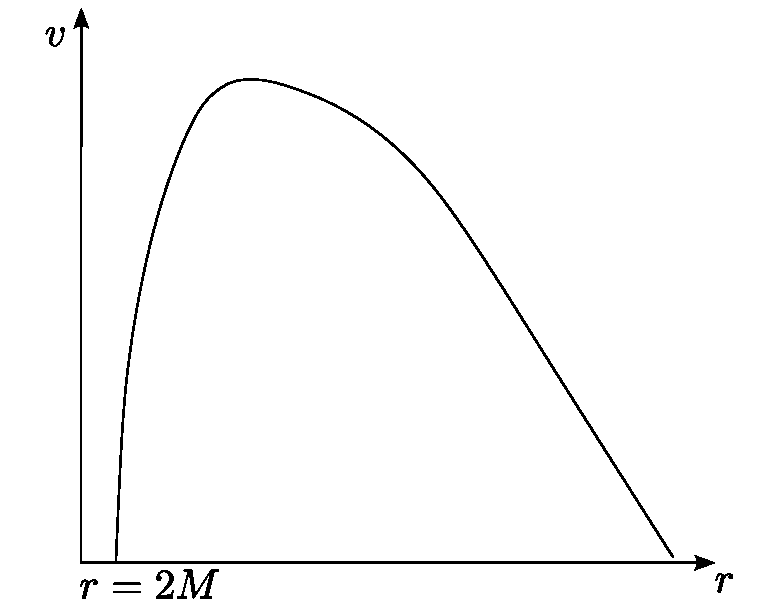
\includegraphics[width=\textwidth]{fig_15-7.pdf}
\captionof{figure}{Schematic plot of the variation of velocity as a function of radial distance from the center for an object falling in from a huge distance. \label{fig:falling}}
%\end{center}
\end{Figure}




What do the shell observers living at shells close to the horizon see? In problem \refproblem{prob:falling} you show that  the velocity of the falling object as observed by the shell observer at distance $r$ (at the moment when the object passes the shell) is given by
\[
v_\sh=-\sqrt{\frac{2M}{r}},
\]
We see that shell observers closer and closer to the horizon will always observe a larger and larger local velocity. The shell observers on the shell just above the horizon $r=2M$ sees that $v_\sh\rightarrow-1$, that the velocity of the object approaches the speed of light as the spaceship approaches the horizon. We have seen a huge difference in results: The far-away observer sees that the object falls to rest at the horizon, the local observer close to the horizon sees the object approaching the speed of light. Already from special relativity we are used to the fact that observers in different frames measure different numbers, but this is a really extreme example. What do the freely falling observers in the spaceship see? For the freely falling observers nothing particular at all happens when they pass the horizon. The freely falling observers are always moving from one local inertial frame to the other, but nothing special happens at $r=2M$.

What velocity do local observers measure beyond the horizon? Do they measure a velocity larger than the velocity of light? In a coming lecture we will look a little bit more at motion beyond the horizon, but here we will look briefly at the \ss line element to see if we get some hints.
\[
\Delta\tau^2=\sst \Delta t^2-\frac{\Delta r^2}{\sst}
\]
Exactly at the horizon, the line element is singular. This is not a physical singularity, but what we call a {\it coordinate singularity}. By changing coordinate system, this singularity will go away and one can calculate $\Delta s$ at the horizon without problems. One may understand this easier by looking at the analogy with the sphere: If a function on the sphere contains the expression $1/\theta$ (where $\theta$ is the polar angel being zero at the north pole) it will become singular on the north pole. By changing the coordinate system by defining the north pole at some other point on the sphere, the point of the previuos north pole will not be singular. In this case the function in itself is not singular on the point of the previous north pole, it is the coordinate system which makes the expression singular at this point.

We will now take a look at this line element when $r<2M$. In this case we can write it as
\[
\Delta\tau^2=\frac{\Delta r^2}{\left|1-\frac{2M}{r}\right|}-\left|1-\frac{2M}{r}\right|\Delta t^2
\]
Looking at the sign, the space and time coordinates interchange their roles. This does not directly mean that space and time interchange their roles, but space does attain one feature which we normally associate with time: An inevitable forward motion. In the same way as we always move forward in time, an observer inside the horizon will always move forwards towards the center. No matter how strong engines you have, you cannot stop this motion: you cannot be at rest inside the horizon, always moving forwards towards destruction at the center exactly as we always move forward in time. A consequence of this is that no shell observers can exist inside the horizon. You cannot construct a shell at rest, everything will always be moving. Inside the horizon we cannot measure a local shell velocity, so even if the shell velocity approaches the speed of light at the horizon it does not necessarily mean that we will have a local velocity larger than speed of light inside the horizon. More about this later.

\section{An example: GPS, Global Positioning System}
\label{sect:gps}

\begin{Figure}
%\begin{center}
\centering
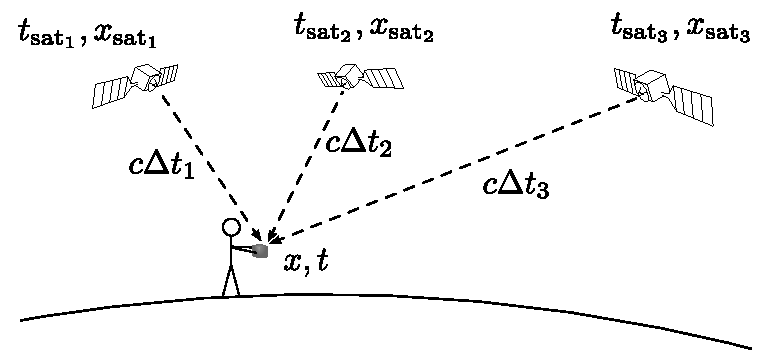
\includegraphics[width=\textwidth]{fig_15-8.pdf}
\captionof{figure}{The GPS system.\label{fig:GPS}}
%\end{center}
\end{Figure}


We have seen that general relativity becomes important for large masses and for distances close to the \ss radius $r\rightarrow2M$. The question now is when we need to take into account general relativistic effects. Clearly this depends on the accuracy required for a given calculation. We will now see one example where general relativity is important in everyday life. The Global Positioning System (GPS) is used by a large number of people, from hikers in the mountain trying to find their position on the map to airplanes navigating with GPS in order to land even in dense fog. GPS is based on 24 satellites orbiting the Earth with a period of 12 hours at an altitude of about 20 000 kilometers. Each satellite sends a stream of signals, each signal containing information about their position $\vec{x}_\mathrm{sat}$ of the satellite at the time $t_\mathrm{sat}$ when the signal was sent. Your GPS receiver receives signals from three satellites (actually from four in order to increase the precision of the internal clock in your GPS receiver, but if your GPS receiver has an extremely accurate clock, only three satellites are strictly necessary: We will for simplicity use three satellites and assume that your GPS receiver contains an atomic clock in this illustration). The situation is illustrated in figure \ref{fig:GPS}. Your GPS receiver contains a very accurate clock showing the time $t$ when you receive the signal. This gives your GPS receiver three equations with the three coordinates of your position $\vec{x}$ as the three unknowns,
\begin{align*}
|\vec{x}-\vec{x}_\mathrm{sat1}|&=c(t-t_\mathrm{sat1})\equiv c\Delta t_1,\\
|\vec{x}-\vec{x}_\mathrm{sat2}|&=c(t-t_\mathrm{sat2})\equiv c\Delta t_2,\\
|\vec{x}-\vec{x}_\mathrm{sat3}|&=c(t-t_\mathrm{sat3})\equiv c\Delta t_3.
\end{align*}
The GPS receiver receives the time $t_\mathrm{sat}$ when a signal was emitted from the satellite. Knowing that the signal travels with light speed $c$ and reading off the time of reception of the signal on the internal clock of the GPS receiver, the receiver can calculate the distance $c\Delta t$ that the signal has traveled. This distance is equal to the difference between your position $\vec{x}$ and the position $\vec{x}_\mathrm{sat}$ of the satellite when the signal was emitted. Solving the three equations above, the GPS receiver solves for your position $\vec{x}=(x,y,z)$ normally expressed in terms of longitude, latitude and altitude. (Note that if a fourth equation were added using a signal from a fourth satellite, another unknown could be allowed: This is how the precision of your GPS clock is increased: your time $t$ is solved from the four set of equations. Here we will assume that your GPS receiver has an atomic clock)

If we assume a simplified one dimensional case, i.e.\ that you only have a one dimensional position $x$, the solution would be
\[
x=c\Delta t\pm x_\mathrm{sat}.
\]
We see that the precision of your calculated position $x$ depends on the precision with which we can calculate the time difference $\Delta t=t-t_\mathrm{sat}$. The signals move with  velocity of 300 000 kilometers per second. If there is an inaccuracy of the order $1{\rm\ \mu s}=10^{-6}{\rm\ s}$, one microsecond, the inaccuracy in the calculated position would be of the order $3\times 10^8{\rm\ m/s}\times10^{-6}{\rm\ s}=300{\rm\ m}$. An inaccuracy of one microsecond corresponds to an inaccuracy of 300 meters in the position calculated by GPS. In such a case GPS would be useless for many of its applications and more seriously, the airplane missing the tarmac with 300 meters would crash!

We know that due to special relativity, the clocks in the satellite and the clocks on Earth (in your GPS receiver) run at different paces because of the relative motions of the satellites with respect to you. We also know from general relativity that the clocks in the satellite run at a different pace than your clock because of difference in distance from the center of attraction (center of Earth). If the clocks in the satellites and the clocks in the GPS receivers were synchronized at the moment when the satellites were launched into orbit, the question is how long does it take until the relativistic effects make the Earth and satellite clocks showing so different times that GPS has become useless. Relativistic effects are usually small so one could expect that it would take maybe thousands of years. If this were the case, we wouldn't need to worry. But remember that we require a precision better than $1{\rm\ \mu s}$ here. This could make relativistic effects important. Let's check.

We start by the gravitational effect. We consider two shells, shell 1 is the surface of the Earth situated at radial distance $r_1=6000{\rm\ km}$ (approximately, we are only looking for orders of magnitude here, not exact numbers). Shell 2 is the orbit of the satellites at radial distance $r_2=6000 + 20000 {\rm\ km}$. A time interval $\Delta t_1$ on the surface of the Earth is related to a time interval $\Delta t$ of the far-away observer by (see equation \ref{eq:tt})
\[
\Delta t_1=\sqrt{\left(1-\frac{2M}{r_1}\right)}\Delta t.
\]
Similarly, a time interval $\Delta t_2$ measured on the satellite clock is related to the far-away time $\Delta t$ by
\[
\Delta t_2=\sqrt{\left(1-\frac{2M}{r_2}\right)}\Delta t.
\]
Dividing these two equations on each other we find that
\[
\Delta t_1=\sqrt{\frac{1-\frac{2M}{r_1}}{1-\frac{2M}{r_2}}}\Delta t_2.
\]
This is the difference in clock pace between the satellite and Earth clocks taking into account only gravitational effects. We will first check the order of magnitude of these terms. What is the mass of the Earth measured in meters? We have 
\begin{align*}
&M_{\rm Earth}=6\times10^{24}{\rm\ kg}\\
&=6\times10^{24}\times(7.42\times10^{-28}{\rm\ m})=0.0044 {\rm\ m}.
\end{align*}
(in case you have forgotten: go back and check how to go from kg to meters). So the term $2M/r$ is of the order $10^{-8}$ for Earth, very much smaller than 1. Thus we can use Taylor expansions,
\begin{align*}
\sqrt{1-x}&\approx1-\frac{1}{2}x+...\\
1/\sqrt{1-x}&\approx1+\frac{1}{2}x+...
\end{align*}
giving for $x=2M/r$
\[
\Delta t_1=\Delta t_2+\left(\frac{M}{r_2}-\frac{M}{r_1}\right)\Delta t_2,
\]
where we have skipped terms of second order in small quantities (two $x$ multiplied with each other) as these are much smaller than the terms of first order in $x$. We see that $\Delta t_1<\Delta t_2$ as expected: Observers far away from the central mass see that clocks close to the central mass run slower. Observers far away from Earth will observe that it takes longer than one second on their wristwatch ($\Delta t_2$) for the clocks on Earth ($\Delta t_1$) to move one second forward.

Inserting numbers for $r_1$ and $r_2$ we obtain
\[
\Delta t_1\approx\Delta t_2-7\times10^{-10}\Delta t_2.
\]
We see that after about one day $\Delta t_2=3600\times24{\rm\ s}$, the satellite clocks are 60 microseconds ahead of the Earth clocks. This corresponds to uncertainties in position measurements of the order 20 kilometers. Thus, one day after launching the satellites, GPS would be useless unless relativistic effects are taken into account!

In order to be sure about this, we need to also look at special relativistic effects. Seen from Earth, satellite clocks (which send time signals read from their own clocks to Earth) go slower (since they are moving with respect to the observers on the surface of the Earth). We have
\[
\Delta t_1^\mathrm{SR}=\gamma\Delta t_2^{SR},
\]
where SR stands for special relativity. In this case $\Delta t_1^{SR}>\Delta t_2^{SR}$ opposite of the general relativistic effect. We need to check whether this effect might be just large enough to cancel the general relativistic effect. From Kepler's 3rd law for the satellite we have (check that you can actually derive this), 
\[
\left(\frac{2\pi r_2}{v_{\phi2}}\right)^2=\frac{4\pi^2 r_2^3}{GM_\mathrm{Earth,kg}}
\]
(using conventional units) we find that the orbital speed of the satellite is $v_{\phi2}=1.3\times10^{-5}$ (dimensionless velocity). In addition an observer at the surface of the Earth moves with velocity (due to Earth's rotation)
\[
v=\frac{2\pi r_1}{24{\rm\ h}}=0.5{\rm\ km/s}
\]
or $v_{\phi1}=1.5\times10^{-6}$ in dimensionless units. The velocity of the satellite relative to the observer on the ground is thus approximately $v_{\phi}=v_{\phi1}+v_{\phi2}\approx1.5\times10^{-5}$ giving $\gamma\approx1+10^{-10}$. In one day we find that the satellite clocks run about 10 microseconds slow (check that you agree), by far not enough to cancel the general relativistic effect. Both effects need to be taken into account in order to make GPS of any use at all, and in order to not make your airplane crash when landing in fog.

We have so far used approximate general and special relativistic expressions separately. Using the \ss line element we may take both effects into account simultaneously and obtain a more accurate expression. Writing first the line element (between two clock ticks) for the observer on the surface of the Earth, we have
\[
\Delta\tau^2=\Delta t_1^2=\left(1-\frac{2M}{r_1}\right)\Delta t^2-r_1^2\Delta\phi_1^2,
\]
where $\Delta r_1=0$ since the observer stays at the same radial distance. We can express this as
\[
\left(\frac{\Delta t_1}{\Delta t}\right)^2=\left(1-\frac{2M}{r_1}\right)-v_{\phi1}^2,
\]
where $v_{\phi1}$ is the tangential velocity of the Earth observer, $v_\phi=rd\phi/dt$ (did you get this transition?). Using the same arguments, we get the same expression for the satellite
\[
\left(\frac{\Delta t_2}{\Delta t}\right)^2=\left(1-\frac{2M}{r_2}\right)-v_{\phi2}^2,
\]
where $v_{\phi2}$ is the tangential velocity of the satellite. Dividing these two expressions on each other, we have
\[
\left(\frac{\Delta t_1}{\Delta t_2}\right)=\sqrt{\frac{1-\frac{2M}{r_1}-v_{\phi1}^2}{1-\frac{2M}{r_2}-v_{\phi2}^2}}.
\]
For low velocities and small $2M/r$ this expression reduces to the approximate expressions above. Note that we have not been very careful when measuring the tangential velocities: We did not specify tangential velocity with respect to which time, Earth time, Satellite time or far-away time. In turns out that taking into account these differences gives corrections to the correction which are so small that they can be ignored. We also did not specify whether the radial distances we used for Earth and the satellite were in \ss coordinates $r$ or in shell distances $r_\mathrm{shell}$. Also these differences are so small that they can be ignored in this case.



%\section{Exercise to be presented on the blackboard: Deriving the Scwarzschild line element.}

%The setting up Einstein's field equations for general relativity and solving them go beyond the scope of AST1100/, but we can still make an argument for why 
%the Schwarzschild line element is plausible as a description of the spacetime 
%outside a spherical mass distribution.  In the following you can assume 
%that all gravitational fields are weak, and that all speeds are negligible 
%compared to the speed of light in vacuum, $c$.  A point mass $m$ is dropped infinitely far from $M$ with 
%zero speed initially. (See figure \ref{fig:fig1}).    

%\begin{Figure}
%\centering
%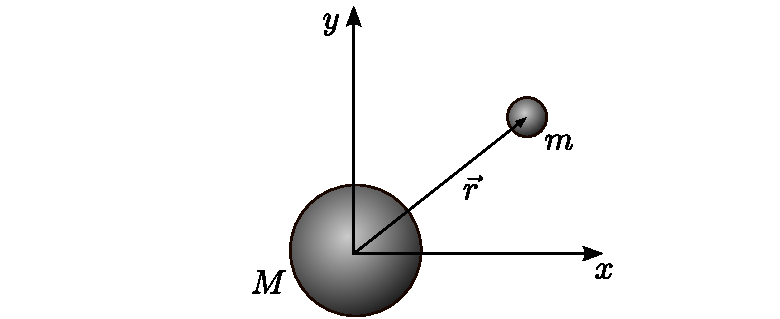
\includegraphics[width=\textwidth]{fig_15-9.pdf}
%\captionof{figure}{A sketch of the situation in this problem. \label{fig:fig1}}
%\end{Figure}


%\begin{itemize}
%\item[a)] Show that the velocity of the point mass in position $\vec{r}$ 
%is given by 
%\begin{equation}
%\vec{v} = -\sqrt{\frac{2GM}{r}}\vec{e}_{r},
%\label{eq:eq1}
%\end{equation}
%where $\vec{e}_r$ is the unit vector in the direction of $\vec{r}$.  
%\item[b)] Consider a free-float system attached to the point mass with 
%coordinates $(t_{\rm FF},x_{\rm FF},y_{\rm FF},z_{\rm FF}) = (t_{\rm FF}, 
%\vec{x}_{\rm FF})$.  Explain briefly why the line element in this system 
%is 
%\[
%ds_{\rm FF}^2 = -c^2dt_{\rm FF}^2+d{\vec{x}}^2 _{\rm FF}.
%\]
%\item[c)] Consider a rigid coordinate system fixed to the stars infinitely 
%far from the mass distribution, $(t_{\rm r},x_{\rm r},y_{\rm r},z_{\rm r})$. 
%Explain why the transformation between this system and the free-float 
%system in the previous point is given by 
%\begin{align}
%dt_{\rm FF} & =  dt_{\rm r} \nonumber \\
%d\vec{x}_{\rm FF} & =  d\vec{x}_{\rm r} + \vec{v}dt_{\rm r}, \nonumber 
%\end{align}
%where $\vec{v}$ is given by equation (\ref{eq:eq1}).  
%\item[d)] Show that the line element in the rigid reference frame is 
%given by 
%\[
%ds_{\rm r}^2 = -\left(c^2-\frac{2GM}{r}\right)dt_{\rm r}^2+2\sqrt{\frac{2GM}{r}}
%dr_{\rm r}dt_{\rm r} + d\vec{x}_{\rm r}^2.
%\]
%\end{itemize}

%It can be shown that this line element is an {\it exact} solution of 
%Einstein's field equations in the empty space outside the spherical 
%mass distribution, expressed in the so-called Painlev\'{e}-Gullstrand 
%coordinates.  Adopting spherical spatial coordinates and dropping 
%subscripts we have 
%\[
%ds^2 = -\left(c^2-\frac{2GM}{r}\right)dt^2 
%+2\sqrt{\frac{2GM}{r}}drdt +dr^2 +r^2(d\theta^2+\sin ^2 \theta d\phi ^2).
%\]
%We can write this line element in a more familiar form by transforming 
%to a new time coordinate, $t_{\rm S}$: 
%\[
%t_{\rm S}=t-\left[\frac{2r}{c}\sqrt{\frac{2GM}{rc^2}}-\frac{4GM}{c^3}
%\tanh ^{-1} \left(\sqrt{\frac{2GM}{rc^2}}\right)\right]
%=t_{\rm S}(t,r).
%\]
%\begin{itemize}
%\item[e)] Carry out the transformation of the line element.  Do you recognize 
%the result?  (Hint: Use the fact that $dt_{\rm S}=\frac{\partial t_{\rm S}}
%{\partial t}dt+\frac{\partial t_{\rm S}}{\partial r}dr$.)
%\end{itemize}

\newpage


\TileWallPaper{51.5pt}{11.5pt}{noisy_grid.png}
\section{Exercises}
\newcounter{problem}
\newcommand{\newproblem}[1]{\refstepcounter{problem}\label{#1}{\bf Exercise \refproblem{#1}}}

\newproblem{prob:rdoppler}

You need to read sections \ref{sect:geometry} - \ref{sect:coordinates} before doing this exercise. Imagine a shell observer at shell $r$ is pointing a laser pen radially outwards from the central mass. The beam has wavelength $\lambda$. Here we will try to find the wavelength $\lambda'$ observed by the far-away observer.
\begin{enumerate}
\item The frequency of the light emitted by the laser pen is $\nu=1/\Delta t$. The frequency of the light received by the far-away observer is $\nu'=1/\Delta t'$. Here $\Delta t$ and $\Delta t'$ is the time interval between two peaks of electromagnetic waves. Show that the difference in time interval measured by the two observers is given by
\[
\Delta t'=\frac{\Delta t}{\sqrt{\sst}}.
\]
{\bf Hint:} Imagine that a clock situated at shell $r$ ticks each time a peak of the electromagnetic wave passes.
\item Use this fact to show that the gravitational 'Doppler' formula, i.e.\ the formula which gives you the wavelength observed by the far-away observer for light emitted close to the central mass, is given by
\[
\frac{\Delta\lambda}{\lambda}=\frac{\lambda'-\lambda}{\lambda}=\frac{1}{\sqrt{\sst}}-1
\]
\item Show that for distances $r\gg2M$ this can be written as
\[
\frac{\Delta\lambda}{\lambda}=\frac{M}{r}
\]
{\bf Hint:} Taylor expansion.
\item We will now study what wavelength of light that an observer far away from the Sun will observe for the light with the wavelength $\lambda_\mathrm{max}=500{\rm\ nm}$ emitted from the solar surface.
\begin{enumerate}
\item Find the mass of the Sun in meters (using that the solar mass is $2\times10^{30}$kg)
\item Find the ratio $M/r$ for the surface of the Sun.
\item Find the redshift $\Delta\lambda/\lambda$ measured by a far-away observer.
\item Is the apparent color of the Sun changed due to the gravitational redshift?
\item For light coming from far away and entering the gravitational field of the Earth, an opposite effect is taking place. The light is blue shifted. Find the ratio $M/r$ for the surface of the Earth.
\item Find the gravitational blue shift $\Delta\lambda/\lambda$ for light arriving at Earth (note: now the light is coming into the gravitational field instead of travelling out out it, what difference does that make in point 1 above?). Does this change the apparent color of the Sun?
\end{enumerate}
\item A quasar is one of the most powerful sources of energy in the universe. The quasars are thought to be powered by a so-called accretion disc: Hot gas circling and falling into a black hole. The gas reaches velocities close to the speed of light as it approaches the horizon, but since we only see the sum of the radiation coming from all sides of the black hole, we expect the Doppler effect due to the velocity of the gas to cancel out. Assume that we find evidence for an emission line at $\lambda=2150$~nm in the radiation from a quasar. Assume also that we recognize this emission line to be a line which in the laboratory is measured to occur at $\lambda=600$~nm. Find from which distance $r$ (expressed in terms of the black hole mass $M$) from the center, the radiation is emerging and Give some arguments explaining why this observation supports the hypothesis of quasars having a black hole in the center. Assume that the Doppler effect due to the quasar's movement with respect to us has been subtracted.
\item Imagine you are a shell observer living at a shell at $r=2.01M$ very close to the horizon of a black hole of mass $M$. Can you use optical telescopes to observe the stars around you? What kind of telescope do you need?
\end{enumerate}

\vspace{0.5cm}

\newproblem{schedules}

Go to MCAst and load the xml corresponding to this exercise, you and your partner should agree on who does which frame.
Both of you are situated in a fixed position around a black hole, one of you in a satellite next to a planet very close to the \ss radius, the other in a lonely space ship a little bit further away from the black hole. You are sending light signals to each other, telling the other when you wake up, when you have breakfast, lunch and dinner and when you brush your teeth and finally when you go to bed. Your task is to find at what time your colleague does this on her/his clock. On your own satellite position, a note appears every time when {\bf you} are getting up, having breakfast etc.

In the upper left corner the clock time on your clock is shown (do not use the upper time showing seconds, only the clock time). Also the mass of the black hole as well as the distance from the center of the black hole for both observers are given. The observer far away from the black hole has a view to the black hole as well as to the planet. The observer close to the black hole is in orbit just above the surface of the planet and is looking outwards towards the other observer.

Assume that the clocks of both observers are synchronized when the videos begin. Assume further that both observers can be treated as shell observers.

\begin{enumerate}
\item Calculate the mass of the black hole in meters
\item Write down the days, hours and minutes for each message you get from your colleague, from the first message in the morning, to the last one at night. One of the observers will see these messages repeated many times, it suffices to use the first sequence of messages.
\item Convert all times to minutes.
\item You are supposed to transform time intervals from one shell observer to the other. In the text you have deduced a formula to transform between a shell observer and the far-away observer, not between shell observers. What we do is to use the far-away observer as a global clock: Now transform the time of all the events to the clock of the far-away observer.
\item Use the times you calculated on the far-away clock to transform to the clock of your colleague.
\item Write these times in terms of hours and minutes. Is your colleague an early riser?
\item Now meet your colleague from the other space ship and check her/his actual schedule. We accept errors of the order 20-30 minutes.
\end{enumerate}







\vspace{0.5cm}

\newproblem{prob:momcons}

You need to read section \ref{sect:maxaging} before doing this exercise.
In this exercise we will use the principle of maximal aging to deduce the law of conservation of angular momentum in general relativity. In the text you have seen three examples of this kind of derivation and here we will follow exactly the same procedure. Before embarking on this exercise, please read the examples in the text carefully.

\begin{Figure}
%\begin{center}
\centering
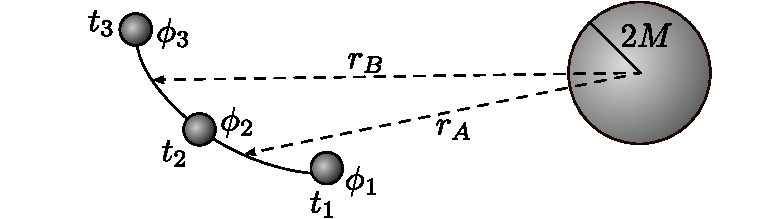
\includegraphics[width=\textwidth]{fig_15-10.pdf}
\captionof{figure}{A sketch of problem 2. \label{fig:L}}
%\end{center}
\end{Figure}

\begin{enumerate}
\item Use figure \ref{fig:L} in this exercise: We will study the motion of an object which passes through three points $(r_1,\phi_1)$, $(r_2,\phi_2)$ and $(r_3,\phi_3)$ at times $t_1$, $t_2$ and $t_3$. We fix $t_1$, $t_2$, $t_3$, $r_1$, $r_2$ and $r_3$ as well as $\phi_1$ and $\phi_3$. The free parameter here is $\phi_{2}$. We assume that between $(r_1,\phi_1)$ and $(r_2,\phi_2)$ the radius is $r=r_A$ (we assume the distance between these two points to be so small that $r$ is constant) and between $(r_2,\phi_2)$ and $(r_3,\phi_3)$ we have $r=r_B$ (see again figure \ref{fig:L}). Use the \ss line element to show that the proper time interval from $\phi_1$ to $\phi_3$ can be written as
\begin{align*}
&\Delta\tau_{13}=\tau_{12}+\tau_{23}=\\
&\sqrt{\left(1-\frac{2M}{r_A}\right)t_{12}^2-\frac{r_{12}^2}{1-\frac{2M}{r_A}}-r_A^2\phi_{12}^2} \\ 
& \qquad +\sqrt{\left(1-\frac{2M}{r_B}\right)t_{23}^2-\frac{r_{23}^2}{1-\frac{2M}{r_B}}-r_B^2\phi_{23}^2}
\end{align*}
\item Use the principle of maximal aging to show that
\[
\frac{r_A^2\phi_{12}}{\tau_{12}}=\frac{r_B^2\phi_{23}}{\tau_{23}}
\]
\item Use this to argue that
\[
r^2\frac{d\phi}{d\tau}
\]
is a conserved quantity.
\item Show that his quantity can be written as
\[
\gamma_\mathrm{shell}rv_\phi
\]
using shell observer speed and tangensial velocity $v_\phi$.
\item Show that this is equivalent to classical spin per mass, $L/m$, in the limit where velocities are small.


\end{enumerate}

\vspace{2cm}


\newproblem{prob:falling}

You need to read section \ref{sect:falling} before doing this exercise. We will leave an object at rest at a large distance from the central mass. We leave the object with velocity zero $v=0$ at a distance so large that we can let $r\rightarrow\infty$. The energy per mass of the particle is then only the rest energy of the particle, $E=m$.
\[
\frac{E}{m}=\sst\frac{dt}{d\tau}=1
\]
\begin{enumerate}
\item Reorganizing this expression find a relation between $dt$ and $d\tau$.
\item Now use a well-known relation between proper time and the space time interval $ds$ as well as an appropriate expression for this interval to show that
\[
\left(\frac{dr}{dt}\right)^2=\sst^2\frac{2M}{r}.
\]
\item Show that the velocity of the falling object at a distance $r$ from the central mass is given by
\[
v=-\sst\sqrt{\frac{2M}{r}}.
\]
\item Use the transformation equations for time and radial distance between the far away observer and shell observer to show that the velocity of the falling object as observed by the shell observer at distance $r$ (at the moment when the object passes the shell) is given by
\[
v_\sh=\frac{dr_\sh}{dt_\sh}=-\sqrt{\frac{2M}{r}},
\]
\end{enumerate}


\newproblem{prob:fallingspaceship}

Go to MCAst and load the xml corresponding to this exercise, you and your partner should agree on who does which frame.
In one frame, the planet frame,  you are positioned in a satellite close to a planet which orbits a black hole at a distance of 1AU. The satellite is not moving with respect to the planet. Another space ship is falling freely radially inwards towards the black hole having a velocity $v$ at the moment when it is passing you. It is emitting blue light signals (seen from the falling space ship frame) with a fixed time interval (in the falling space ship frame) between each signal. In the other frame, the falling frame, you are positioned in the falling space ship, looking at your friend positioned close to the planet who is sending red light signals (seen from the planet frame) with a fixed time interval (in the planet frame) between each signal.

The mass of the black hole, the locally observed shell speed of the falling space ship at 1 AU from the black hole as well as the time interval between each signal in the frame which emits the signal is given in the upper left corner.

{\bf Important:} As in most other xml-videos in this course, the light travel time from the objects to the camera is not considered, meaning that you see all events instantaneously. This would correspond to an infinite light speed for light travelling from the objects/events to the camera. In the videos in this exercise, this effect is more visibile than in most other videos. In part 2E you will learn how light speed is changed in a gravitational field and in exercise 2E.2 you will continue this exercise taking into account the real light speed.

\begin{enumerate}
\item Characterize each of the two observers as either far away observer, shell observer of freely falling observer.
\item Use the general expression for $E/m$ as well as some known transformation relations between far-away and shell quantities to show that the energy of the falling space ship can be written as
\[
\frac{E}{m}=\sqrt{1-\frac{2M}{r}}\gamma_\sh
\]
where $\gamma_\sh$ corresponds to the locally osberved shell velocity at a distance $r$ from the black hole. Remember that you may use a local intertial frame, and thereby special relativity, during a short moment when the space ship passes the shell observer.
\item Calculate the energy per mass $E/m$ of the falling space ship.
\item Combine the \ss line element with the expression for energy to show that the relation between a time interval $\Delta\tau$ in the falling space ship and a time interval $\Delta t$ on the far-away-clock, can be written as
\[
\Delta\tau = \frac{1-\frac{2M}{r}}{E/m}\Delta t
\]
\item Use the relation between far-away-time and shell time to find a relation between a time interval in the falling space ship, $\Delta\tau$, and a time interval in the planet frame, $\Delta t_\mathrm{shell}$.
\item We will now use this expression to find the distance $r$ between the space ship and the centre of the black hole during the time between two emitted signals. You may have observed that the emitted light changes colour due to gravitational red/blue shift. We could have used the colour alone to determine the distance, but here we will ignore the colour and only use the observed period between the emitted signals. You know that in the frame from which the signals are emitted, the light signals are emitted with a constant known time interval between each signal. {\bf For the planet frame:} find the distance $r$ from the black hole to the falling space ship in the time period between the observed violet and green signal as well as between the observed blue and red signal. Assume the time interval between two signals to be so short that the distance $r$ can be assumed constant during this interval. Give the answer in units of AU and in units of \ss radii. Use both numbers to judge whether your answer may be reasonable or not (give arguments). {\bf For the falling frame:} find your own distance $r$ from the black hole in the time period between the observed red and yellow signal as well as between the blue and the violet signal. Assume the time interval between two signals to be so short that the distance $r$ can be assumed constant during this interval. Give the answer in units of AU and in units of \ss radii. Use both numbers to judge whether your answer may be reasonable or not (give arguments).
\item Repeat the previous calculation, but now use the two last signals that you receive. How close to the \ss radius was the space ship at that point?
\item Before you meet to compare videos, can you imagine how this looks from the other observer? Use the equations that you already found to argue. Now meet to compare.
\item After meeting, you should discuss the result seen from the space ship frame: the time interval between each received light interval seems to grow shorter and shorter as you approach the horizon. Can this really be? What will happen as you hit the horizon? Is the video correct? If not, what is wrong?
\end{enumerate}





\newproblem{prob:stepbystep}

\begin{Figure}
%\begin{center}
\centering
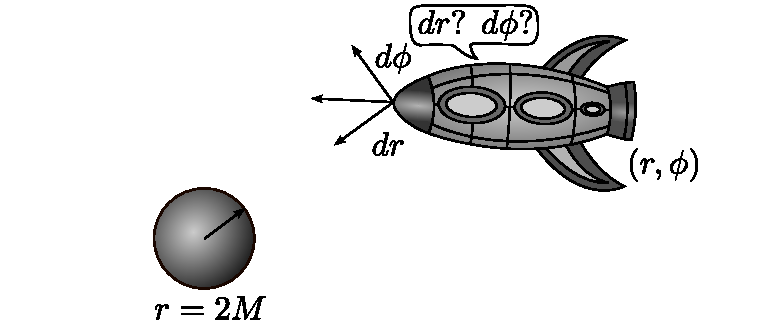
\includegraphics[width=\textwidth]{fig_17-1.pdf}
\captionof{figure}{The spaceship is out of fuel. The engines stop. What will be the next movement in $r$ and $\phi$ direction? \label{fig:stepbystep}}
%\end{center}
\end{Figure}

It will be very difficult to do this exercise withtout having read sections \ref{sect:geometry} - \ref{sect:falling} first.
In figure \ref{fig:stepbystep} we show a spaceship at position $(r,\phi,t)$ in \ss coordinates around a black hole of mass $M$. The spaceship has used all its fuel and can therefore not use its engine, it is falling freely.  We will now study the motion of the spaceship step by step. We will ask the question, what is the new position $(r,\phi,t)$ in \ss coordinates of the spaceship after a time interval $\Delta\tau$ has passed on the wrist watches of the astronauts? By increasing $\Delta\tau$ and thereby the other coordinates step by step, we will be able to follow the motion $(r,\phi)$ of the spaceship.
\begin{enumerate}
\item We will start by finding an expression for the increase in far-away time $\Delta t$ when the time on the astronauts wrist watch increases by $\Delta\tau$. This is basically the transformation between far-away time and time as measured by the freely falling observer. Show that
\[
\Delta t=\frac{E/m}{\sst}\Delta\tau.
\]
where $E/m$ is energy per mass of the space ship.
\item Show that after a proper time interval $\Delta\tau$, the space ship has moved an angle
\[
\Delta\phi=\frac{L/m}{r^2}\Delta\tau.
\]
where $L/m$ is the total angular momentum per mass of the space ship.
\item We have already obtained the displacements $\Delta\phi$ and $\Delta t$ per proper time interval $\Delta\tau$. Now we need to find the radial displacement $\Delta r$. Using the two previous expressions, the relation between proper time and space time interval as well as an appropriate expression for $\Delta s$, show that
\begin{align*}
&\Delta r=\\
&\pm\sqrt{\left(\frac{E}{m}\right)^2-\left[1+\left(\frac{L/m}{r}\right)^2\right]\sst}\Delta\tau.
\end{align*}
\end{enumerate}

\newproblem{prob:aircrew}

This exercise will be much easier if you read section \ref{sect:gps} first.
Assume that the crew on an airplane works on average 8 hours per day 365 days a year for 50 years. Assume that all this time, they are at a height of $\Delta r=10$ km above the ground (assume the radius of the Earth to be $r=6000$~km) moving at a velocity of $v_\mathrm{Airplane}=1000$ km/h with respect to the center of the Earth. We will here ignore the effect of acceleration during take-off and landing.
\begin{enumerate}
\item Show that proper time intervals $\Delta\tau$ for the crew at work can be written in terms of time intervals $\Delta t_\mathrm{Earth}$ measured on Earth clocks as
\[
\frac{\Delta\tau}{\Delta t_\mathrm{Earth}}=\sqrt{\frac{1-\frac{2M}{r+\Delta r}-v_\mathrm{Airplane}^2}{1-\frac{2M}{r}-v_\mathrm{Earth}^2}},
\]
where $v_\mathrm{Earth}$ is the velocity of a person on the Earth with respect to the center of the Earth.
\item This expression may give numerical problems when using very small numbers. For this reason we will try a Taylor expansion. Calculate $M/r$ as well as the velocity $v_\mathrm{Airplane}$ and $v_\mathrm{Earth}$ (use Earth's rotation period) in dimensionless units. Are these so small that we can Taylor expand the expression above in terms of $2M/r$, $v_\mathrm{Airplane}$ and  $v_\mathrm{Earth}$?
\item Show that the Taylor expansion of this expression, assuming that these three quantities are small, can be written as
\begin{align*}
&\frac{\Delta\tau}{\Delta t_\mathrm{Earth}}\approx\\
&1+\frac{1}{2}(v_\mathrm{Earth}^2-v_\mathrm{Airplane}^2)+M\left(\frac{1}{r}-\frac{1}{r+\Delta r}\right).
\end{align*}
{\bf Hint:} Taylor expand first in 
\[
x=-(\frac{2M}{r+\Delta r}+v_\mathrm{Airplane}^2),
\]
then in 
\[
y=-(\frac{2M}{r}+v_\mathrm{Earth}^2).
\]
\item Use this expression to find how much shorter a crew member lives with respect to persons staying on Earth, taking into account only relativistic effects?
\item Would you now skip next year's vacation in the fear of getting old too fast?
\end{enumerate}

\vspace{0.5cm}

\newproblem{prob:gps}

Study carefully section \ref{sect:gps} on GPS. Now open the xml file corresponding to this exercise in MCAst. There is just one common file from one frame of reference.

In the video, you are situated at a fixed point, somewhere at the equator of a planet. The mass and radius of the planet is given in the upper left corner of the video. Two GPS satellites are passing above you in the sky, continously sending messages about the (x,y) position and time (measured on the satellite clock) specifying when and where the signal was sent. The satellites go in a circular orbit around equator. Since all positions, both for the satellite and observer are at the equator, we will use a 2-dimensional (x,y) system to denote all positions. The origin of the system is the center of the planet. During the video, the camera is fixed at your position, but the camera angle changes so that it follows the two satellites. Note that you even receive signals from the satellite when they are below the planet.

We assume that your planet clock and the satellite clocks are synchronized at the beginning of the video. {\bf Important:} the planet clock is the time shown in the second line in the upper left corner, {\bf you should not use the upper clock in this exercise.} You main task in this exercise is to use the signals sent from the satelittes to determine your (x,y) position on the planet.

In this exercise, precision is of high importance. In order to get consistent results, you need to use the values of constants which were used to create this video, these are $c = 299792.458$km/s for the velocity of light and $G=6.67\times10^{-11}$ for the gravitational constant. {\bf In all your calculations you need to use all digits given, this is also the case for all times and positions which you find in the video.}. If you omit some digits you loose the necessary precision in order to see the small effects of general relativity. We will assume that the planet is not rotating, meaning that your (x,y) position is fixed.

\begin{enumerate}
\item Use information given in the video to find the height of the orbit of the satellites.
\item Use information from the video as well as some celestial mechanics to fint the orbital velocity of the satellites.
\item Now choose a very early moment in the video, one of the very first frames which are displayed: Write down the position and time signals which you receive from both satellites at this moment. You must also write down current time at the planet (second clock, not the upper one) at this moment when you receive the signals. Use this information to infer your (x,y) position. You have been given some hints already in this chapter on how you can use the time it takes for the light signal to arrive and the relation to the distance to the satellite. Remember that the time sent from the satellite is the time when the satellite sent the signal, whereas the planet time is the time when you receive the signal. For the moment, please ignore all relativistic effects. You need to combine some analytical calculations with some simple numerics and clever thinking to be able to deduce your position. {\bf Two more hints:} (1) Assume the position of the satellite is given by $\vec{r}_\mathrm{sat}$ and your position is $\vec{r}$. Then you know how to write $|\vec{r}_\mathrm{sat} - \vec{r}|$ in terms of $\Delta t$. You also know how to write $|\vec{r}_\mathrm{sat} - \vec{r}|$ in terms of the angle $\alpha$ between $\vec{r}_\mathrm{sat}$ and $\vec{r}$. And when you find this angle you're almost done. (2) You can easily check if you answer is correct: check if the left and right hand side of your equations are equal using your solution.
\item Now you should take into account relativistic effects: both the gravitational and special relativistic effects should be included. You know that the clocks onboard the satellites tick with a different rate that your clock. In order to get your correct position, you need to derive the time when these signals were sent measured on the planet clock. Use your GR knowledge to find the times when the signals were sent from the satellite in the planet frame.
\item Now use your new times to find your position. With how many meters did you miss your position?
\item Now you should pick a moment towards the end of the video, preferably one of the very last frames of the video. Repeat all the previous exercises in order to find your position with and without correction for relativistic effects.
\item You should have found a considerably larger deviation in the latter case. Why? What would happen if you repeated your position estimate in a few days? Would GPS still be useful?
\end{enumerate}

\end{multicols}


\end{document}

